\documentclass[a4paper,twoside]{danarticle}
\usepackage{a4}
\usepackage[pdftex]{color}
\usepackage[pdftex]{graphicx}
\pagestyle{headings}
\usepackage{amsthm}
\usepackage{german}
\selectlanguage{english}
\usepackage[pdftex,colorlinks=true,
                      pdfstartview=FitB,
                      linkcolor=blue,
                      citecolor=blue,
                      urlcolor=blue,
		      bookmarks=true
          ]{hyperref}
\pdfinfo{
            /Title      (DoorStep: A system for visitor awareness)
            /Author     (Daniel Hahn)
            /Keywords   (Visitors)
}
\newtheorem{definition}{Definition}
\theoremstyle{remark}
\newtheorem*{example}{Example}
\sloppy

\begin{document}

  \begin{titlepage}
    \raggedleft
    \vspace{2cm}
    \sffamily
    {\huge
    DoorStep: A System For Visitor Awareness\\
    }
    {\large
    Daniel Hahn\\
    }
    \vspace{2cm}
    \raggedright
    {\Large
    \hspace{2cm}Studienarbeit\\
    }
    {\large
    \hspace{2cm}Institut f\"ur Telematik, Universit\"at Karlsruhe\\
    \hspace{2cm}Computing Department, Lancaster University\\
    }
    \vspace{1cm}
    \begin{center}
      \includegraphics[width=2cm]{tecologo}
      \hspace{1cm}
      \includegraphics[width=2cm]{lancslogo}
    \end{center}
    \vspace{5cm}
    {\normalsize
    \hspace{2cm}Betreuer/Supervisor: Prof. Dr. Wilfried Juling \\
    \hspace{2cm}Betreuer/Supervisor (Lancaster): Prof. Hans Gellersen \\
    \vspace{5mm}
    \hspace{2cm}Betreuender Mitarbeiter/Coordinator: Albrecht Schmidt \\
    }
    \vspace{2cm}
    {\normalsize
    \hspace{2cm}Anmeldung/Started: Jan 2002 \\
    \hspace{2cm}Abgabe/Completed: Mar 2002 \\
    }
    \vspace{4cm}
    \centering
    {\small 
    Dank an/Thanks \\
    Kristof v. Laerhoven, Martin Strohbach, Chris Needham \& Team \\
    The people and staff at the Lancaster Computing Department \\
    }
  \end{titlepage}
  \newpage
  \tableofcontents
  \newpage
  \begin{abstract}
    {\selectlanguage{german}
    In den vergangenen Jahren ist das World Wide Web zu mehr als einer
    Sammlung statischer Dokumente geworden. Es ist heute 
    ein \emph{sozialer Raum}, in dem die \glqq Netzbewohner\grqq\ virtuelle 
    \glqq Orte\grqq\ 
    aufbauen, sich gegenseitig \emph{besuchen} und an anderen sozialen
    Aktivit"aten teilnehmen.
    
    Es kann angenommen werden, dass die Gastgeber (hosts) dieser 
    \glqq Pl"atze\grqq\ 
    ein gro"ses Interesse daran h"atten die Aktivit"at in ihrem
    Online-\emph{Territorium} zu beobachten - wenn es denn eine einfache
    M"oglichkeit dazu g"abe.
    
    Erste Arbeiten von Gellersen und Schmidt\cite{webaware} f"uhrten zu der Idee
    von \emph{Blicken in die Besucherseiten (Glances into visitors site's)}. Bei
    diesem Ansatz wurden die (bereits vorhandenen) Protokolldateien der
    Webserver analysiert, um die Seiten der Besucher zu finden und diese dem
    Gastgeber auf einem separaten Bildschirm zu pr"asentieren. Der Gastgeber soll
    dadurch ein verbessertes Bewusstsein f"ur die Vorg"ange auf seinen Seiten 
    erhalten, mehr "uber seine Besucher erfahren und zur Verbesserung seiner
    eigenen Seiten inspiriert werden. Diese Methode geht davon aus, dass fast
    jeder Besucher eine eigene Seite im Netz hat, die (ausgehend von den
    Serverprotokollen) mit einem einfachen Algorithmus gefunden werden kann.
    
    Ziel der vorliegenden Arbeit war, dieses Konzept weiterzuf"uhren und
    einen Ansatz zu entwickeln der sich nicht mehr nur auf das
    Zur"uckverfolgen von Besuchern beschr"ankt, sondern die Zusammenh"ange
    zwischen den Besuchern und verschiedenen Webseiten kennt und ausnutzt.
    Dieses System sollte mit den vorhandenen Besucherdaten (d.h. den
    Serverprotokollen) arbeiten, diese analysieren und dann versuchen eine Reihe
    m"oglichst interessanter Seiten (oder Web-\glqq Pl"atze\grqq) zu finden und
    dem Nutzer zu pr"asentieren.
    
    Bei der Analyse der verf"ugbaren Benutzerdaten und Ressourcen zeigte sich,
    dass dieses System drei Hauptaufgaben erf"ullen muss: 
    
    \begin{itemize}
      \item{Die Analyse der Benutzer\emph{ereinisse}, um etwas "uber den
            Besucher zu erfahren und einen Ansatzpunkt f"ur die weiteren 
            Schritte zu haben}
      \item{Die Suche nach Web-\emph{Pl"atzen}, die in irgendeiner Weise mit
            dem Besucher in Verbindung stehen}
      \item{Eine Auswahl der \emph{interessantesten} dieser Web-\emph{Pl"atze},
            die dann dem Nutzer pr"asentiert werden}
    \end{itemize}
    
    Um die Verbindungen zwischen Web-Pl"atzen finden und verarbeiten zu k"onnen,
    wurde hier das Konzept von \emph{Relationen} eingef"uhrt: Zwei Webseiten
    stehen in einer \emph{Relation} zueinander wenn sie ein sie verbindendes
    Merkmal aufweisen. Dies kann beispielsweise eine gemeinsame DNS-Dom"ane 
    sein, in der sich die Seiten befinden, oder ein Querverweis 
    (\emph{Hyperlink}). Da bereits 
    mehrere Arbeiten gezeigt haben, dass sich u.a. "uber \emph{Hyperlinks} soziale
    Gruppen identifizieren lassen (vgl. Adamic\cite{links}), scheint dieser Ansatz
    sinnvoll um ein virtuelles \emph{Territorium} zu beschreiben. 
    
    Das in dieser Arbeit beschriebene DoorStep-System benutzt ein frei
    konfigurierbares Netzwerk von \emph{Relationsfindern}, um Seiten zu finden
    die mit dem Besucher direkt oder indirekt in Verbindung stehen.
    Ausgangspunkt f"ur diese Suche ist eine einzelne Seite, die in einer
    besonders engen Beziehung zu dem Besucher steht (idealerweise seine eigene
    Heimseite). Aus den so gefundenen Seiten werden dann durch eine
    Bewertungsfunktion die f"ur den Benutzer interessanten ausgew"ahlt und
    pr"asentiert.
   
    Der Hauptaugenmerk beim Entwurf des DoorStep-Systems lag auf einer
    gr"o"stm"oglichen Flexibilit"at: Obwohl hier verschiedene Relationen,
    Suchstrategien und Bewertungsfunktionen exemplarisch vorgestellt werden, 
    sollte das System 
    nicht auf bestimmte Algorithmen festgelegt sein, sondern die M"oglichkeit
    bieten beliebige Herangehensweisen zu testen. Aus diesem Grund definiert das
    DoorStep-System zwar das Zusammenspiel zwischen den verschiedenen
    Komponenten, aber nicht die darin zu verwendenden Algorithmen.
    
    Um das System unter realit"atsnahen Bedingungen testen zu k"onnen, wurde
    die DoorStep-Architektur als Java-basierte modulare Testplattform 
    implementiert. Die Plattform verbindet die einzelnen Module (die in den
    Komponenten des DoorStep-Modells entsprechen) durch ein XML-basiertes Datenformat
    und erlaubt so, neue Relationen und Suchstrategien schnell und einfach zu
    integrieren. Das System wurde an der Lancaster University
    mit den Besucherdaten
    eines aktiven Webservers getestet.
    
    Obwohl im Rahmen dieser Arbeit keine lang angelegte Benutzerstudie
    durchgef"uhrt werden konnte, waren die ersten Testergebnisse
    vielversprechend: Das System fand zumeist Seiten, die im Zusammenhang mit den
    Besuchern standen, und oft das Interesse der Benutzer erregten.
    Die modulare
    Testplattform hat sich bew"ahrt und bildet einen guten Ausgangspunkt f"ur
    weitere Untersuchungen, insbesondere f"ur eine ausf"uhrlichere
    Benutzerstudie.
    }
  \end{abstract}
  \newpage
  \section{Introduction}
    In recent years, the World Wide Web has become more than just a collection
    of static documents, or even a collection of services. It is now perceived
    as a \textit{social space}, where the \textit{netizens} build virtual
    \textit{places}, \textit{visit} each other and engage in all kinds of
    activities.
    
    It can be assumed that the \textit{hosts} of those places would be
    very interested in what is \lq\lq going on\rq\rq\ in their online
    \textit{territory} --- if
    there was a convenient way of monitoring the activity. 
    
    Although
    information about \textit{visits} is readily available in the
    form of web server logs, commercial tools for displaying it (e.g. 
    AWStats\cite{awstats}) will only
    provide statistical information, but do not explore the rich context in which
    the visits took place. 
    
    Initial research into the subject by Gellersen and Schmidt\cite{webaware}
    yielded the
    \textit{glances into visitor's sites} approach. Their assumption was 
    that most of
    the visitors to a site had their own place somewhere on the web, and in
    presenting those places to the host they could give him an understanding of the
    kind of \textit{territory} his place is in.
    
    In this paper we will take this approach a step further: We will argue that
    even if the visitor does not have an own place (or if we are
    simply unable to find it) he will always have \textit{relations} to various
    places, and in exploring different types of relations we may be able to
    explore different types of \textit{territories} that in, some way, is adjacent to
    the host's place.
    
    The notion of \emph{relations} between web places is not an entirely new 
    one: Web communities and relations by hyperlinks have already 
    been the subject of research by Adamic\cite{links},
    Flake\cite{flake}, Gibson\cite{gibson}, 
    Larson\cite{larson} and others. 
    Adamic and Adar, for example, not only found 
    evidence that a hyperlinks indicate a social relations, but also that 
    clusters of hyperlinked pages indicate social groups and can be identified 
    with relative ease\cite{links}. These findings are important for the current work, 
    since they prove that this way of exploring relations is a viable one. The main
    focus of the previous work, however, was to show that meaningful relations 
    between pages exists and to identify groups of related pages. In particular,
    most of the researchers did not suggest any particular application of their
    findings.
    
    The DoorStep system (which we present in this paper), 
    on the other hand, is based on the assumption that 
    meaningful relations between web places do exist, but does not concern itself 
    with their exact nature -- in fact, the system is designed 
    to work with almost all imaginable kinds of relations. What we propose is an 
    efficient way to exploit existing relations, connect them to visits 
    and prepare the results in a way that facilitates presentation.
    
    Our system does also not concern itself with the exact 
    nature of the end user display. While we propose the use of an ambient 
    display (like that used in \cite{ambient}), the system allows for many 
    different ways of displaying the results.
    
    In this paper we will introduce a system for finding places that are 
    \textit{related} to
    visitors (or visits) and we will present the results which were gathered 
    from a first implementation of the system.
  \section{The DoorStep System}
    DoorStep is a system that attempts to find \textit{places} which are somehow
    \textit{related} to \textit{visits}. We assume that each
    of this \textit{places} can be described by an URL of the form described in
    \cite{url}. Furthermore, we will use the naming conventions and definitions
    introduced in \cite{webaware}:
    \begin{center}
    \begin{minipage}{10cm}
    \itshape
    In the web infrastructure, a web place [\dots] is defined as 
    a set of resources in the web. Resources can
    be HTML documents, images, other media objects or arbitrary applications.
    These resources are made available by web servers, i.e. programs that manage
    resources and make them available worldwide through the web protocols. A
    visit to a web place then relates to a request for a resource in the
    designated set. A request originates from a client, i.e. a program the
    visitor uses to specify his request, typically a standard web browser. Web
    servers routinely log requests for resources [\dots]. These server logs
    constitute a rich source on web activity.
    \end{minipage}
    \end{center}
    There are documents (such as \cite{logfile}) that describe in great detail 
    the data available from web server log files. The most important pieces of
    information used in the DoorStep system are:
    \\
    
    \textbf{Client Address:} The network address of the client system to which 
    the requested resources are sent. This is either the IP address of the 
    computer which is the visitor's web browser or, if HTTP proxies are 
    involved, the address of a proxy server. We will also call this the 
    \textbf{visit source}.
    \\
    
    \textbf{Timestamp:} The date and time at which the request was received.
    \\
    
    \textbf{Resource:} A description of the resource that was requested.
    \\
    
    \textbf{User Agent:} A string identifying the visitor's user agent 
    software. This usually consists of the name and version of the browser, 
    crawler or toolkit that made the connection.
    \\
    
    \textbf{Referer:} An URL describing the resource that referred a visitor to
    us. (e.g. the URL of the page that contained the hyperlink to the 
    local page).
    \\
    
    Additionally to
    this \textit{primary} information, data may be gathered from the
    context of the visit: For example, a certain \verb$User-Agent$ header 
    may indicate a certain type of visitor (e.g. a crawler or bot), or a visit
    from a visitor in the \verb$.co.uk$ domain can be assumed to come from
    Britain. Both the primary and secondary information may be used for finding
    relationships.
    \subsection{System overview}
      When the system receives a visit, it will perform the basic processing
      steps shown in Figure \ref{steps_overview}, starting with the 
      attempt to find one or 
      more URLs (or web places) that act as starting points for further 
      processing. These 
      starting points should have a close connection to the original visit since 
      they will represent it during the following steps.
      
      In the following text and definitions, the term \lq\lq URL\rq\rq\ 
      is used as a convenient shorthand for \lq\lq web place\rq\rq . However, 
      these URLs are objects that 
      do not only contain a resource locator, as described 
      in \cite{url}, but \emph{all} information the system has gathered about 
      the web place addressed by that locator. This includes both information 
      about  the resources served from that URL (e.g. document type, hyperlinks) 
      and information retained from the original visit event if the URL is a 
      starting point (e.g. \verb$Referer:$ headers).
      
      The starting points will then be fed into a network of \textit{relation 
      finders} that attempt find URLs of web places that are somehow related to 
      the them. The \textit{relation finder} network is the central part of the 
      system: It follows the implicit and explicit connections that link one 
      place with it's neighbours and thus explores the virtual surroundings of 
      the starting point. 
      
      \begin{figure}[ht]
        \centering
        \includegraphics[width=12cm]{webgraph}
        \caption{The web as a graph}
        \label{webgraph}
      \end{figure}
      The relation finders treat the whole web as a huge graph (Figure
      \ref{webgraph}), of
      which the web places (and other machines) are the vertices. A relation
      between two web places can then be thought of as an edge of the graph,
      connecting those places. Relations can either be directed, like
      hyperlinks, or undirected (e.g. \lq\lq pages are from the same
      organisation\rq\rq). 
      The relation finders will enter the graph at the
      starting vertices found in the first step and from there explores paths to
      neighbouring vertices.
      
      At the end of the relation finding phase, the system will have found a
      cluster of web places, representing the virtual neighbourhood of the
      visitor. Each of them will be rated by a number of \textit{rating
      functions}, in order to determine how interesting they may be to the user.
      The rated places will then be passed on to a display system and presented  
      to the user.
      \begin{figure}[ht]
        \centering
	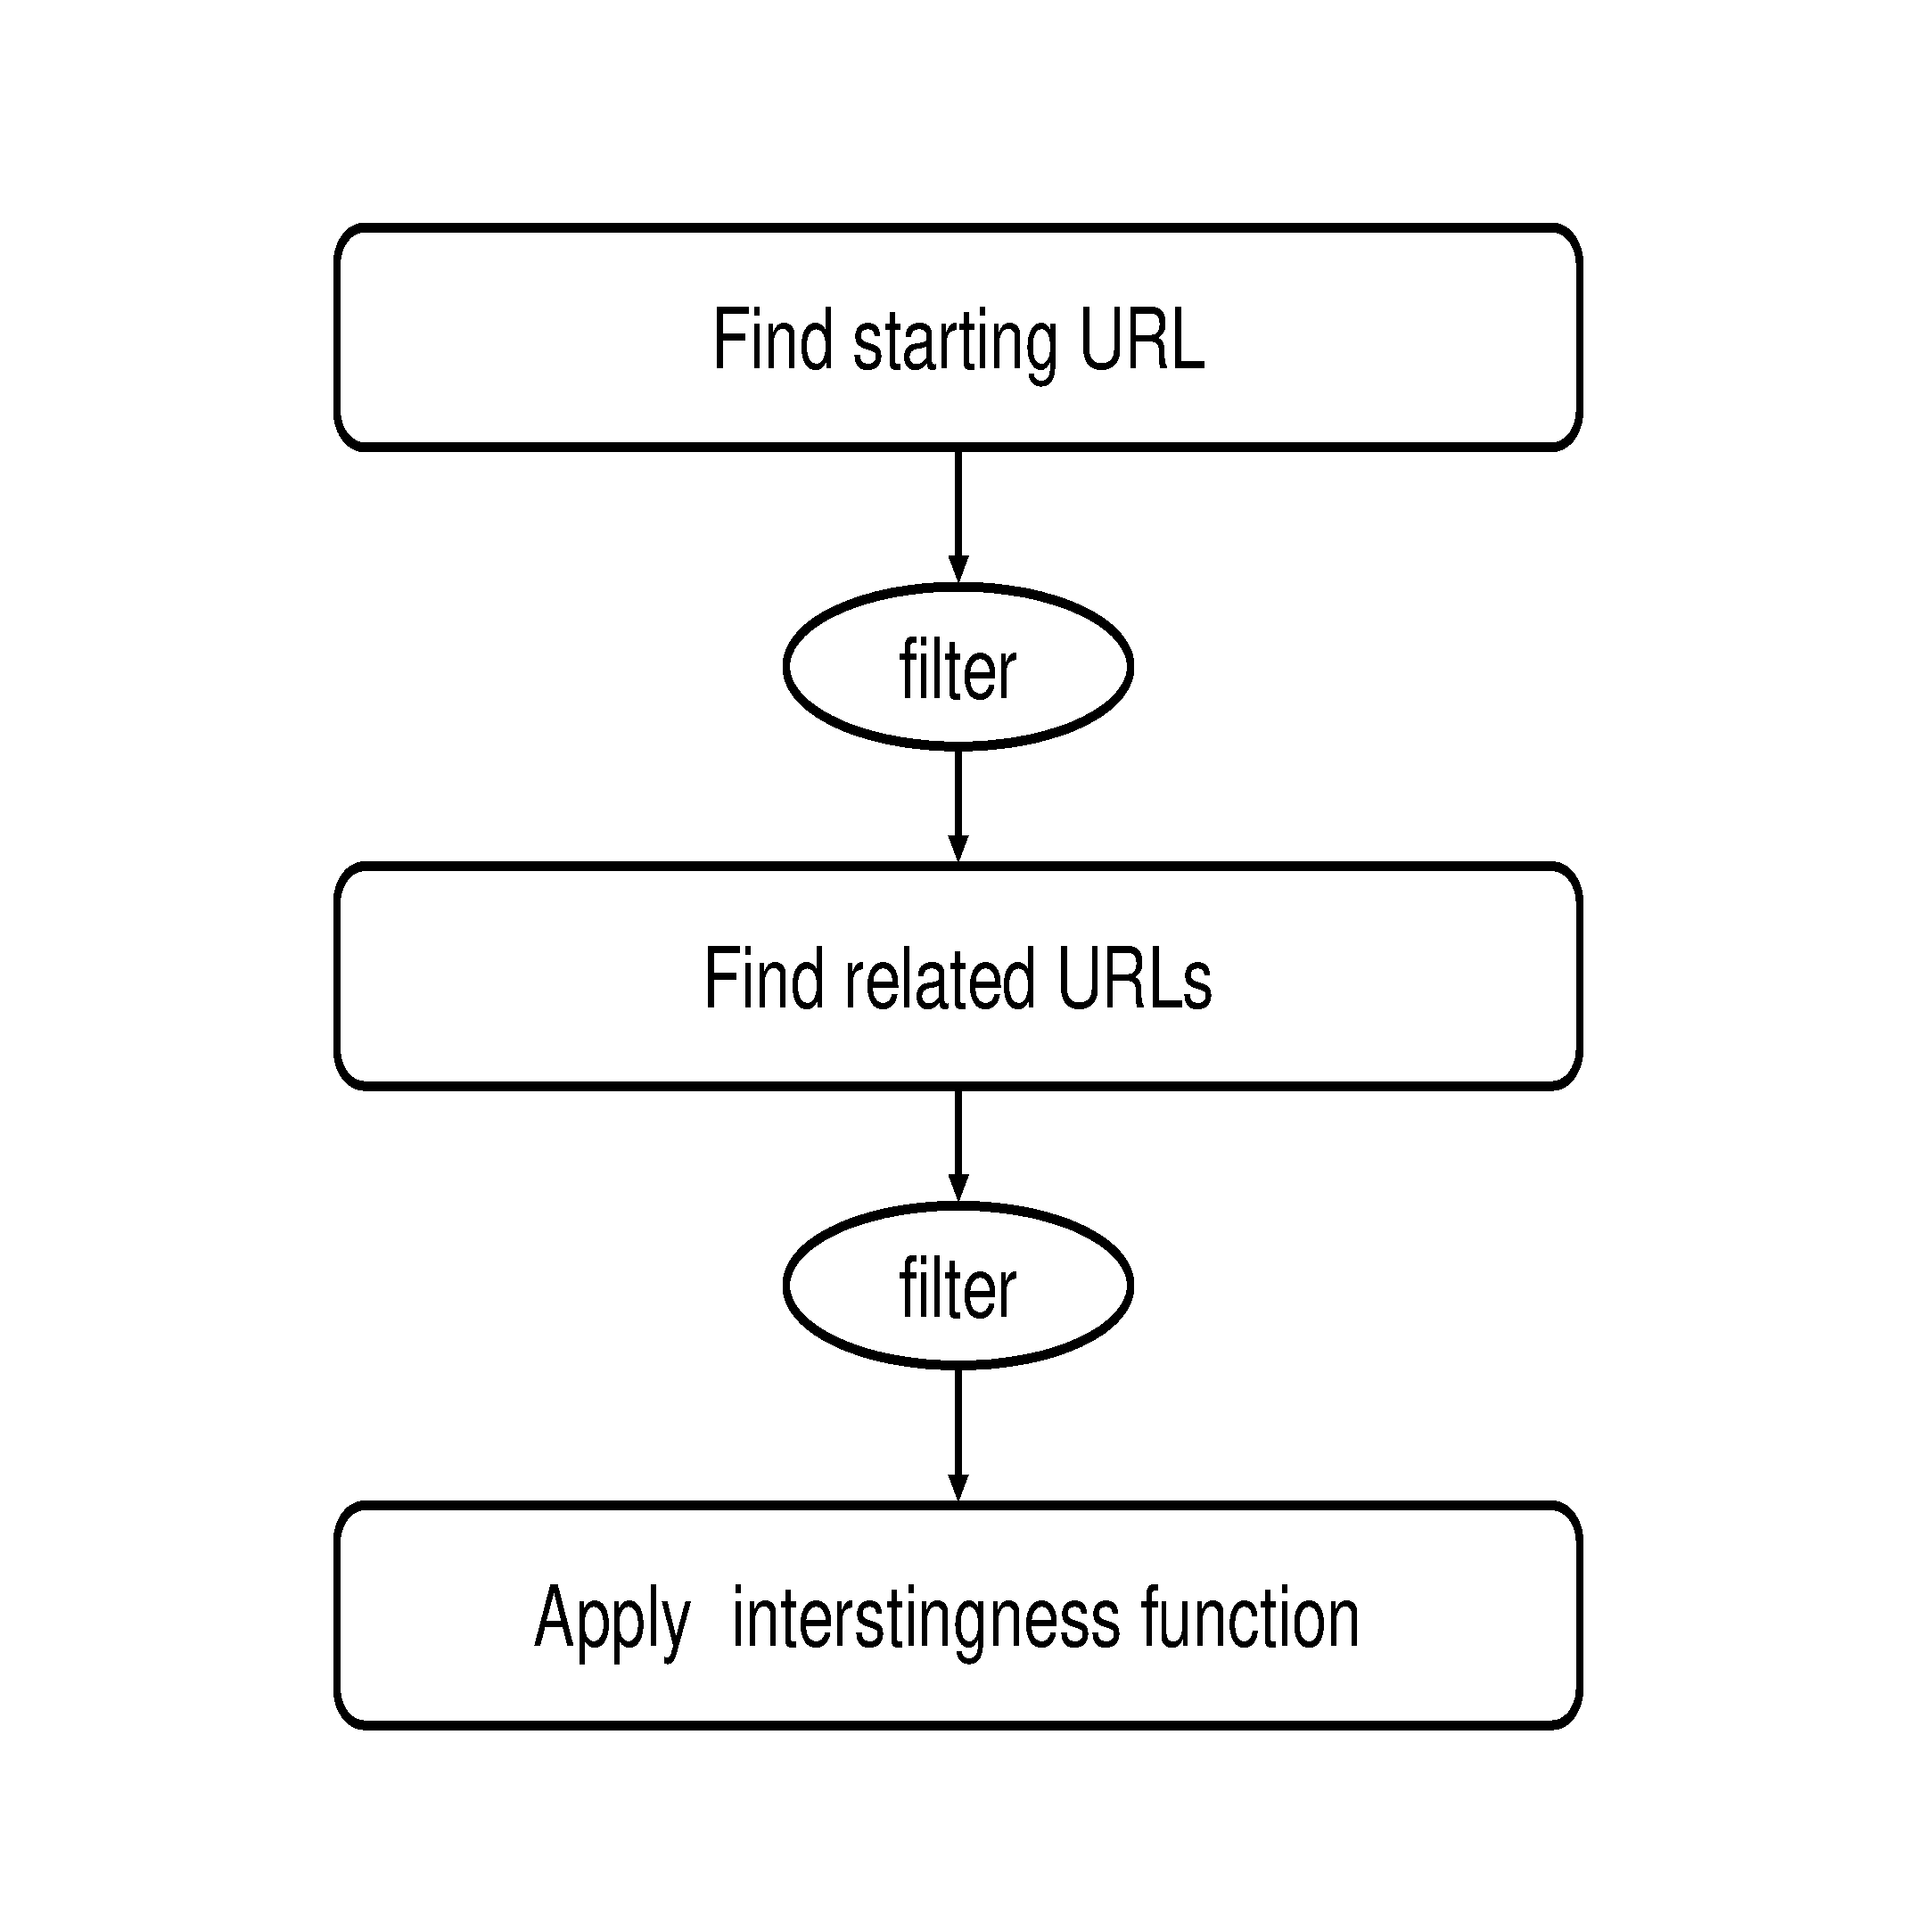
\includegraphics[width=12cm]{steps_overview}
	\caption{Major processing steps of DoorStep}
	\label{steps_overview}
      \end{figure}
    \subsection{Finding starting places}
       \label{findstart}
       \begin{figure}[ht]
       \centering
	 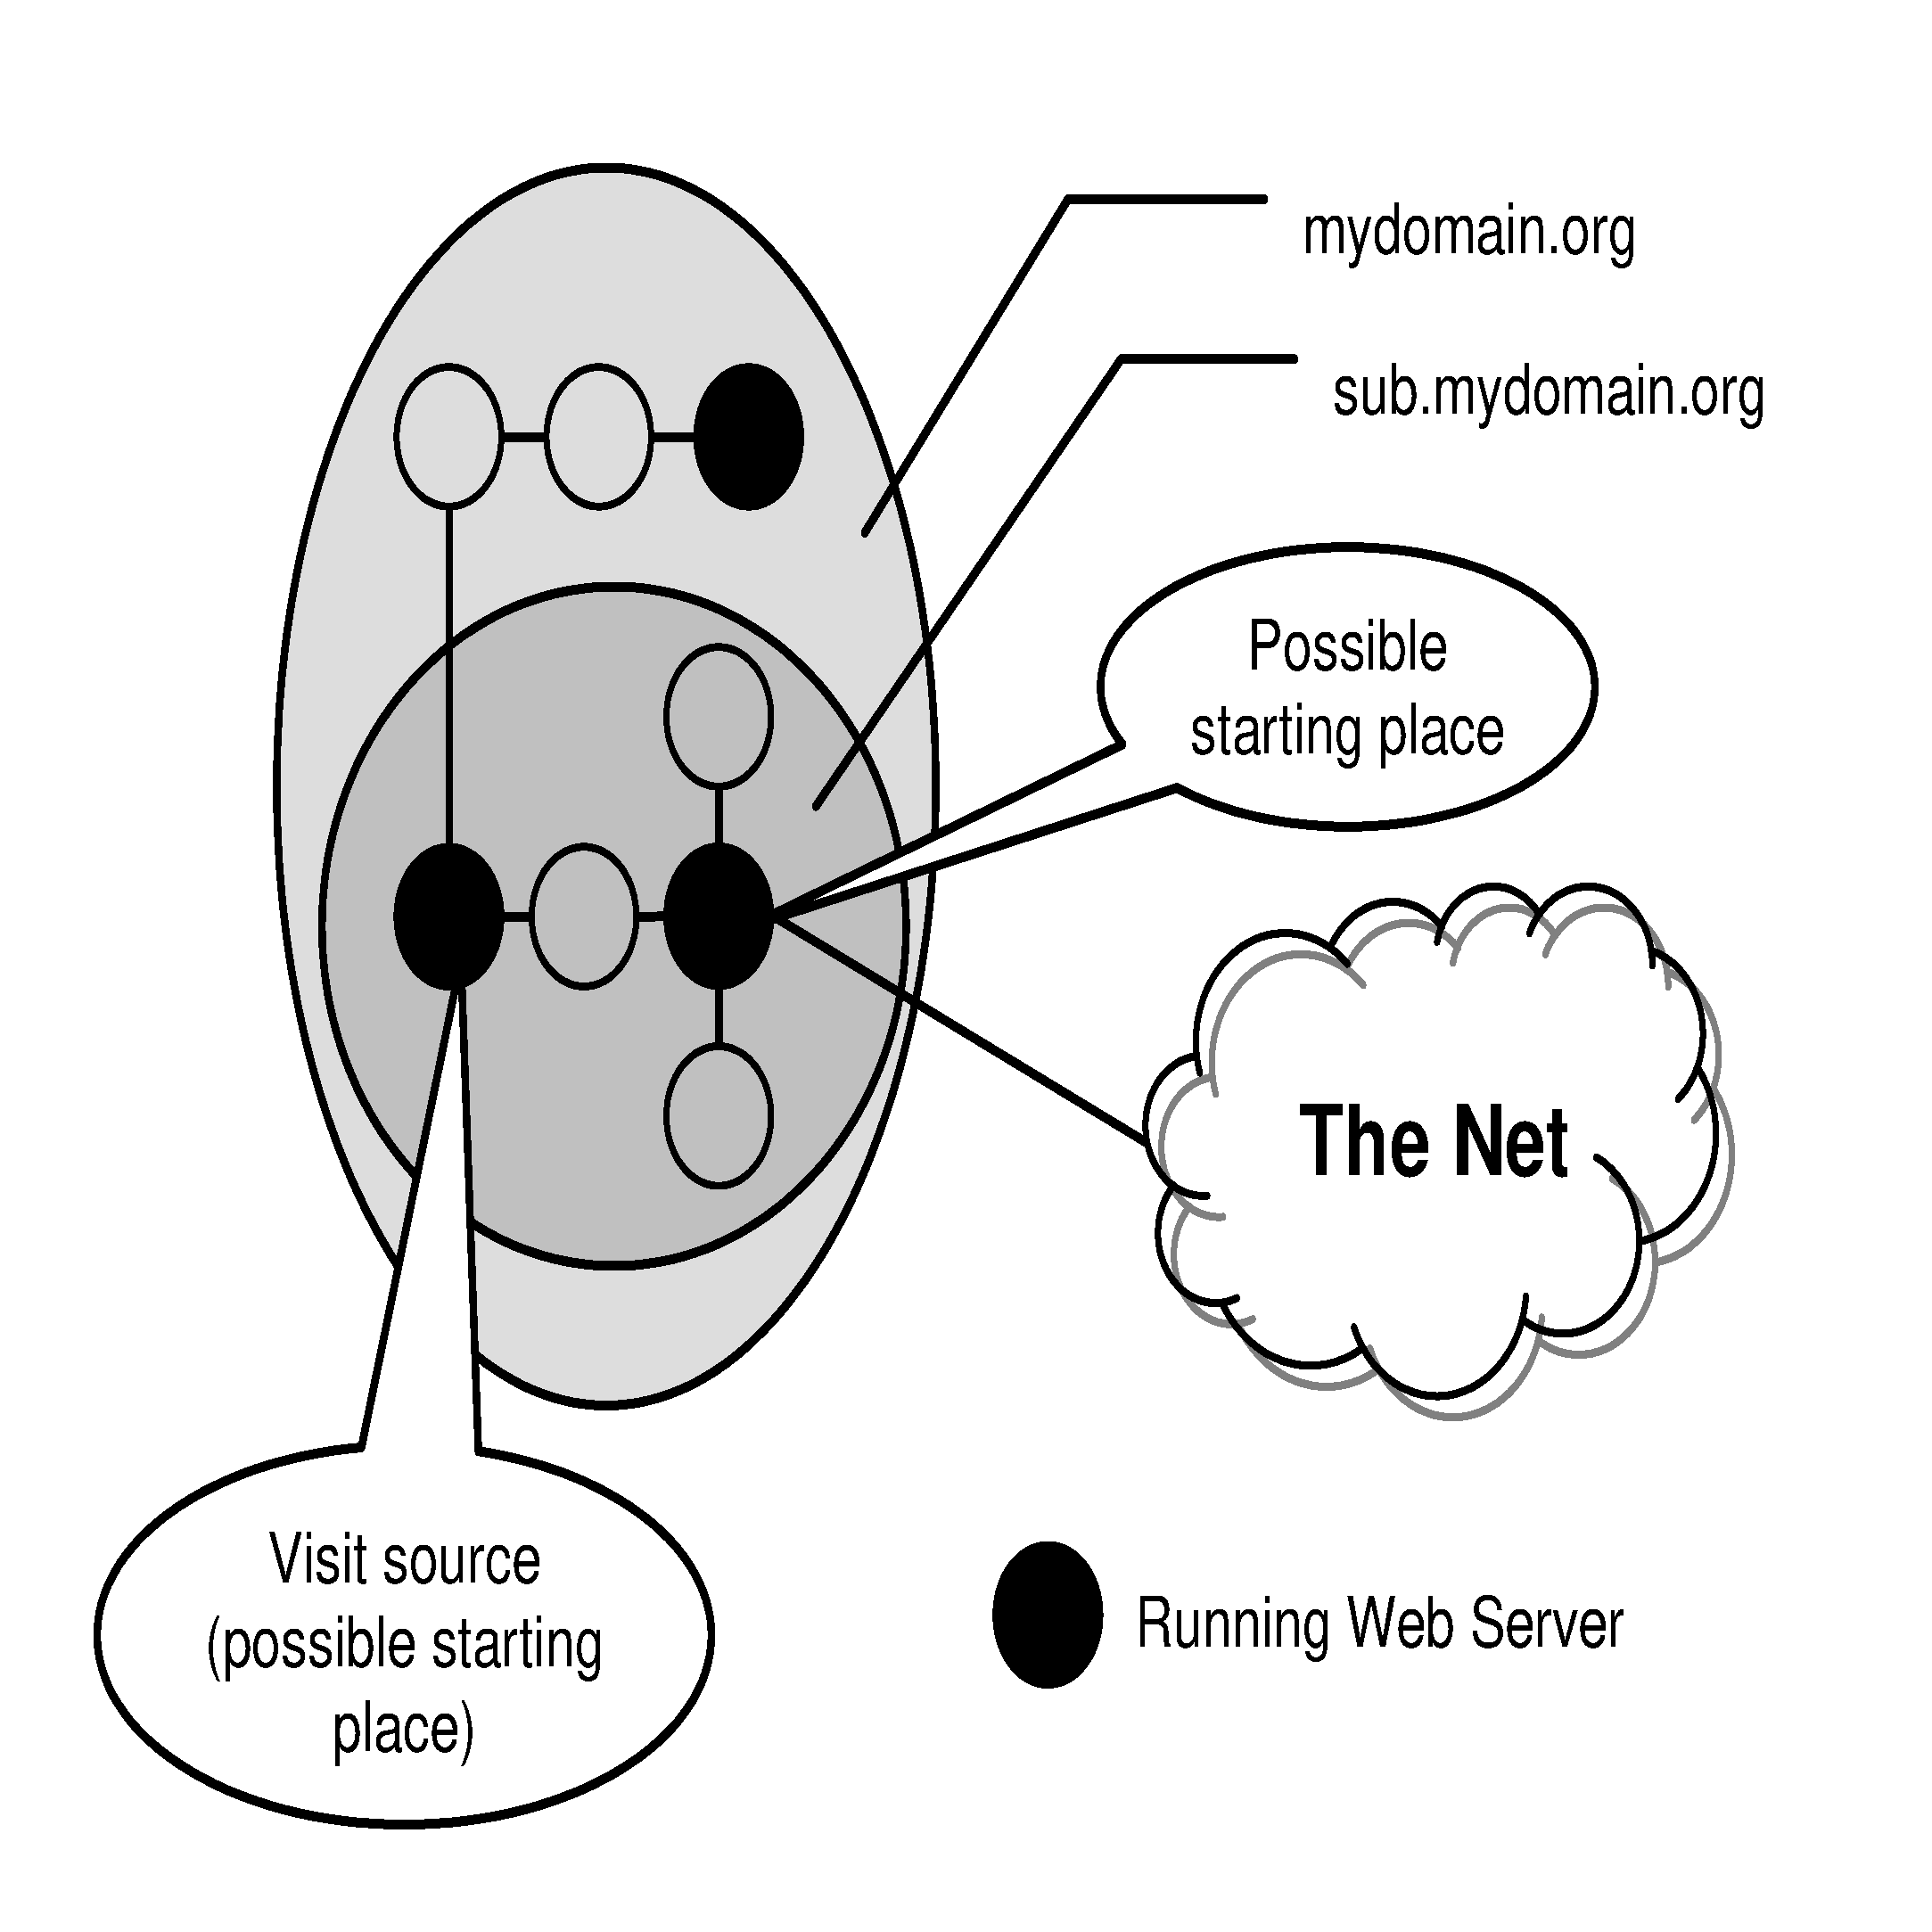
\includegraphics[width=12cm]{startingplace}
	 \caption{Selecting a starting place}
	 \label{startingplace}
       \end{figure}
       \label{startingsection}
       Relations between web places are easy to describe and handle, but relations
       between visits, visitors and places are somewhat harder to
       grasp. To avoid the complications of modelling them, the system
       will pick one (or several) web places that act representatives, or
       proxies, for the visit. These are the \textit{starting points} of the 
       relation finding process,
       in the graph model these are the nodes from which the algorithm will
       start exploring the edges. 
       
       Each starting point must have a close connection to the visit that it is
       meant to represent. In terms of the DoorStep system we demand that a
       starting point should be \textit{as close as possible} to the visit it is
       representing. The metric that measures the \lq\lq distance\rq\rq\ between
       a visit and a web place will vary depending on the type of visit and the
       information at hand, but for HTTP visits (that originate from a network
       address) we use the following metric (also Figure \ref{startingplace}):
       \begin{definition}
       \label{metric}
       Let \verb$a$ and \verb$b$ be two fully qualified DNS host names with the
       subdomain tokens \verb$a_part[]$ and \verb$b_part[]$:
       \begin{center}
        \verb$a$ = \verb$a_part[n].a_part[n-1]. ... .a_part[0]$\\
        \verb$b$ = \verb$b_part[m].b_part[m-1]. ... .b_part[0]$\\ 
       \end{center}
       If $ n \geq m $, and the number of matching right-hand tokens of the two
       names is $ x $ then the distance between \verb$a$ and \verb$b$ is 
       $ n - x $. The number of matching right-hand tokens is the largest number
       $ x $ for which \verb$a_part[y] = b_part[y]$ $ \forall y : 0 \leq y \leq x $.
       \end{definition}
       \begin{example}
       For the hosts with the names \verb$a.b.c$ and \verb$e.d.b.c$  the number
       of matching right-hand tokens is 2 (\verb$b$ and \verb$c$). Since the
       hostname with the most tokens (\verb$e.d.b.c$) has 4 of them, the distance
       between those names is $ 4 - 2 = 2 $.
       \end{example}
       A similar metric can easily be construed for hosts that have no
       qualified DNS name, but only a network (IP) address. We do not give such
       metric here since we found that most of visits sources have a DNS name
       and that those which do not aren't particularly useful for the DoorStep
       processing.
       
       With the given metric, the hostname closest to a
       visit source -- the visit source itself -- 
       is often not really web place because there is no web server
       running at that address; we say that the respective URL is not
       \textit{alive}. Having starting points that are not \textit{alive} can
       be somewhat awkward during the relation finding phase (e.g. if trying to
       follow the hyperlinks from the starting points), and in these cases we
       will attempt to find \textit{alive} starting points using the algorithm
       already used in \cite{webaware} (Listing in Figure \ref{domaintest}):
       
       \begin{itemize}
         \item{If the visit source is alive, copy it to the output}
	 \item{As long as the hostname has more than two tokens, do the
	 following:}
	 \begin{itemize}
	   \item{Try if the new hostname, prefixed with \verb$www.$ is alive.}
	   \item{If it is alive, copy it to the output.}
	   \item{Remove the first token from the hostname.}
	 \end{itemize}
       \end{itemize}
       
       For example, if a visit comes from the host
       \verb$banana.hoogla.boogla.org$, the algorithm would first try that
       host itself (Distance 0), then \verb$www.hoogla.boogla.org$ (Distance 1),
       and finally
       \verb$www.boogla.org$ (Distance 2). If any of those hosts is
       \textit{alive}, it may be used as a starting point. Otherwise
       the algorithm fails.
       \begin{figure}[ht]
       {\ttfamily
       \begin{tabbing}
           \hspace{5mm} \= \hspace{5mm} \= \hspace{5mm} \= \hspace{5mm} \= \\
	   @subdom\_parts = \textit{split}(\verb$/\./$, visit\_source); \\
	   \\
	   \textbf{if} ( \textit{\&alive}(join(\verb$'.'$, @subdom\_parts) \{
	   print OUT @subdom\_parts; \} \\
	   \textbf{for} \verb-( ; $#parts > 0 ; shift(@parts) )- \{ \\
	   \>  \textbf{if} ( \textit{\&alive}(\"www.\" . join(\verb$'.'$,
    	   @subdom\_parts))) \{ \\
	   \> \> print OUT www . @subdom\_parts; \\
	   \> \} \\
	   \} \\
         \end{tabbing}}
	 \caption{Algorithm for selecting alive starting points (Perl)}
	 \label{domaintest}
       \end{figure}
     \subsection{Finding related places} 
       A network of \textit{relation finders} is the central processing unit of 
       the DoorStep system (Figure \ref{relations}). 
       A \textit{relation} finder is an object that will 
       examine a web place (an URL) and attempts to find other URLs that are 
       related to it (remember that URL is used as a synonym for \textit{web
       place}!). 
       \begin{definition}
       An URLs $ u_1 $ is related to another URL $ u_2 $ by some relation 
       $ \rightarrow $
       ($ u_1 \rightarrow u_2 $) if it has some characteristic $ c $ in regard
       to $ u_2 $. The characteristic can usually described by a boolean
       relationship function: $ c = r_{\rightarrow}(u_1, u_2) $:
       \[
         r_{\rightarrow}(u_1, u_2) = \hspace{1mm} \mbox{true} \hspace{2mm} 
	     \Leftrightarrow \hspace{1mm} u_1 \rightarrow u_2
       \]
       $ U_{\rightarrow}(u_x) $ is the set of all URLs that a given URL $ u_x $ 
       is related to (by the relation $ \rightarrow $), and it's members are 
       called the \emph{relatives} of $ u_x $.
       \end{definition}
       In the graph model of the network, this kind of relation is equivalent
       with a directed edge from $ u_1 $ to $ u_2 $, and we say that $ u_1 $ is
       \textit{weakly related} to $ u_2 $. \textit{Strong relations} are
       equivalent to undirected edges.
       Examples of relations include hyperlinks (weak) or web places that are
       within the same DNS domain (strong). 
       \begin{definition}
       Two URLs $ u_1 $ and $ u_2 $ are \emph{strongly related} by a relationship
       $ \rightarrow $ if $ u_1 \rightarrow u_2 $ as well as 
       $ u_2 \rightarrow u_1 $. A relationship $ \leftrightarrow $ is called a
       \emph{strong} relationship if
       \[
         u_1 \leftrightarrow u_2 \Rightarrow u_2 \leftrightarrow u_1 
       \]
       for all possible URLs $ u_1 $ and $ u_2 $. In the case of a strong 
       relationship, $ U_{\leftrightarrow}(u_x) $ will be an equivalency 
       class, and $ \leftrightarrow $ an equivalency relation.
       \end{definition}

       When a relation finder $ F $ examines an URL $ u_x $, it will attempt to 
       find a set of URLs to which $ u_x $ is related by some relation 
       $ \rightarrow_F $. It isn't necessary that the relation finder finds 
       \emph{all} relatives of $ u_x $, a subset of $ U_{\rightarrow_F}(u_x) $ 
       will suffice. Usually, the relation finder will only be able to find 
       all relatives if $ U_{\rightarrow_F}(u_x) $ can be computed from $ u_x $ 
       without further knowledge (e.g. if $ u_x \rightarrow_F u_y $ means 
       $ u_x $ contains a hyperlink to $ u_y $ then $ u_x $ contains all 
       information to compute $ U_{\rightarrow_F}(u_x) $). In all other cases the 
       relation finder will contain a heuristic that selects a set of 
       \textit{candidate} URLs that are possibly related to $ u_x $. From these 
       candidates it will then choose the relatives of $ u_x $. In practice the 
       heuristic will often include the use of a web search engine like 
       Google\cite{google}. Those engines have several properties that make the well 
       suited for relation finding and will be discussed in detail in the next 
       section.
       
       \begin{figure}[ht]
         \centering
	     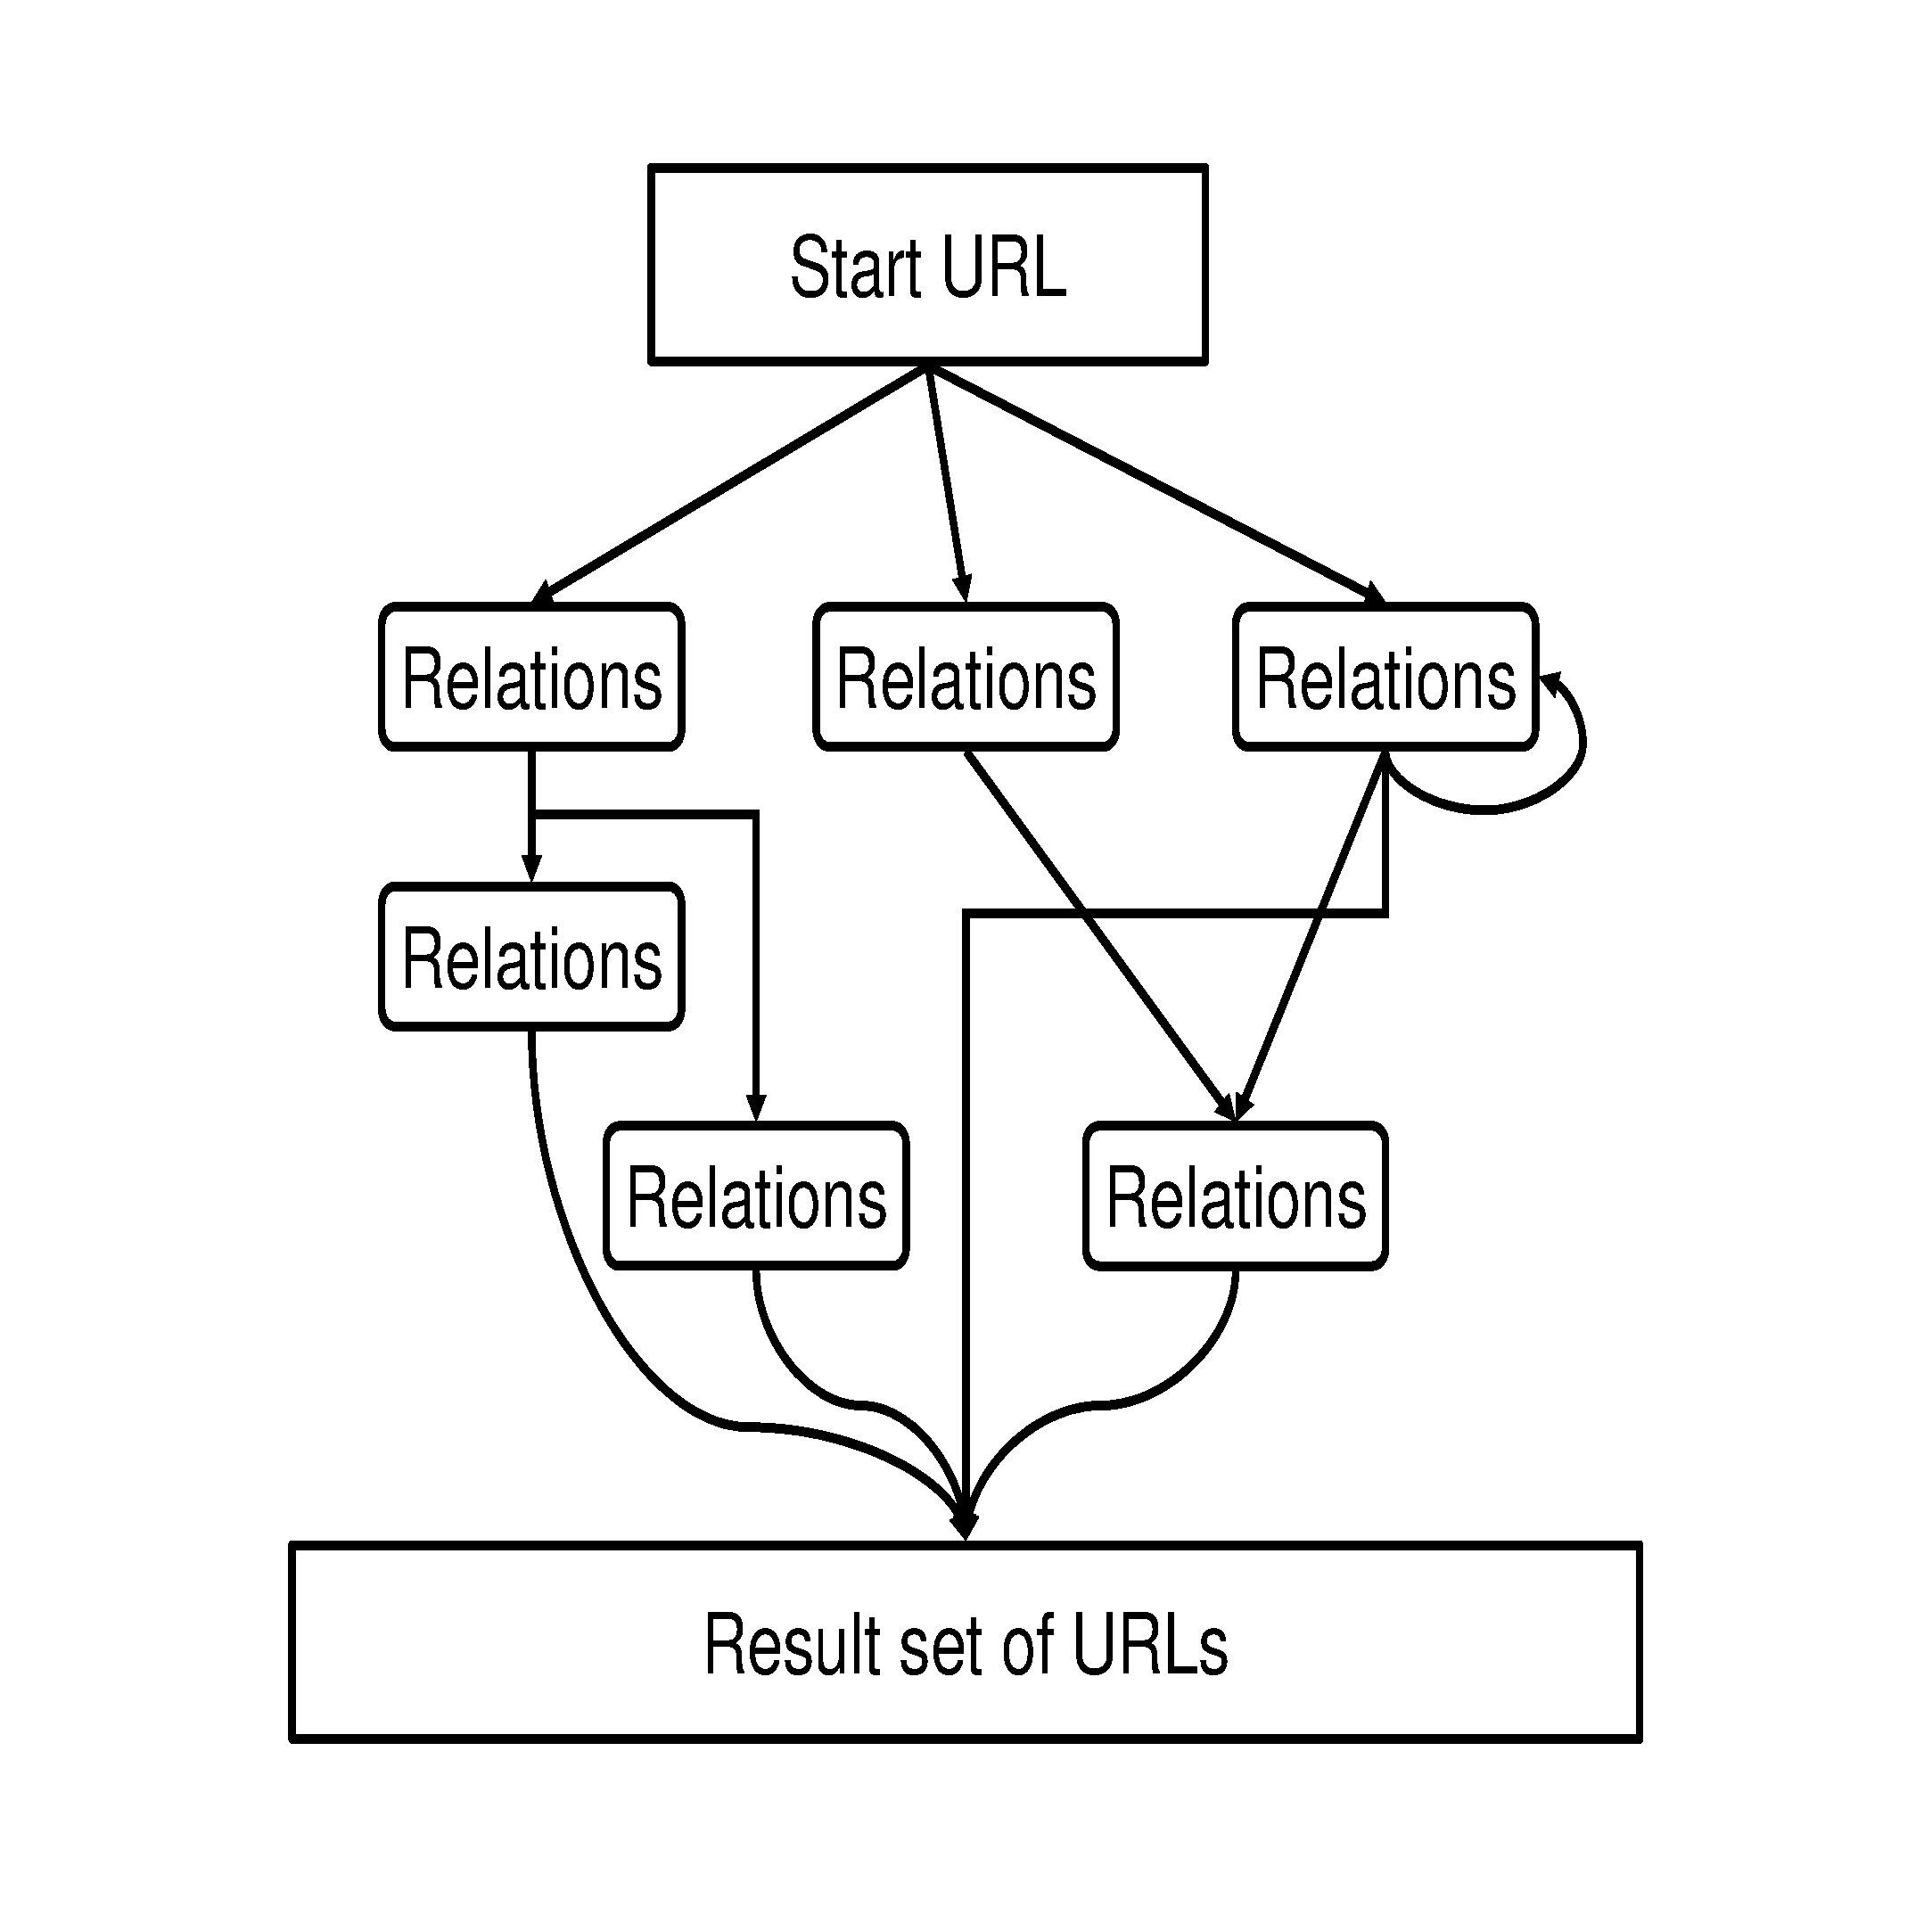
\includegraphics[width=12cm]{relations}
	     \caption{Data flow through different relation finder instances}
	     \label{relations}
       \end{figure}
       
       All the relation finders are arranged in a network structure like shown in 
       Figure \ref{relations}. Each relation finder implements one relationship
       function which it applies to the URLs it receives. A relation finder
       receiving a new URL will try to find a set of relatives (which will often
       include the original URL) and make it available on it's output. The
       output of a relation finder may either be passed on to the output of the
       network or be fed into the input of another relation finder, including
       itself (a relation finder has to ensure that no endless loops are created
       here).
       
       \begin{figure}[ht]
        \centering
        \includegraphics[width=12cm]{relationsteps}
        \caption{Two Relation Finders exploring a Graph}
        \label{relationsteps}
      \end{figure}
       
       In the graph model, a relation finder will work on a single node at a 
       time, attempting to find edges that go from the original node to 
       neighbouring ones (Figure \ref{relationsteps}). 
       The nodes that are found in this way may then then be 
       used as starting points for further relation finders.
     \subsection{Degrees of relationship}
       \begin{figure}[ht]
       \centering
	 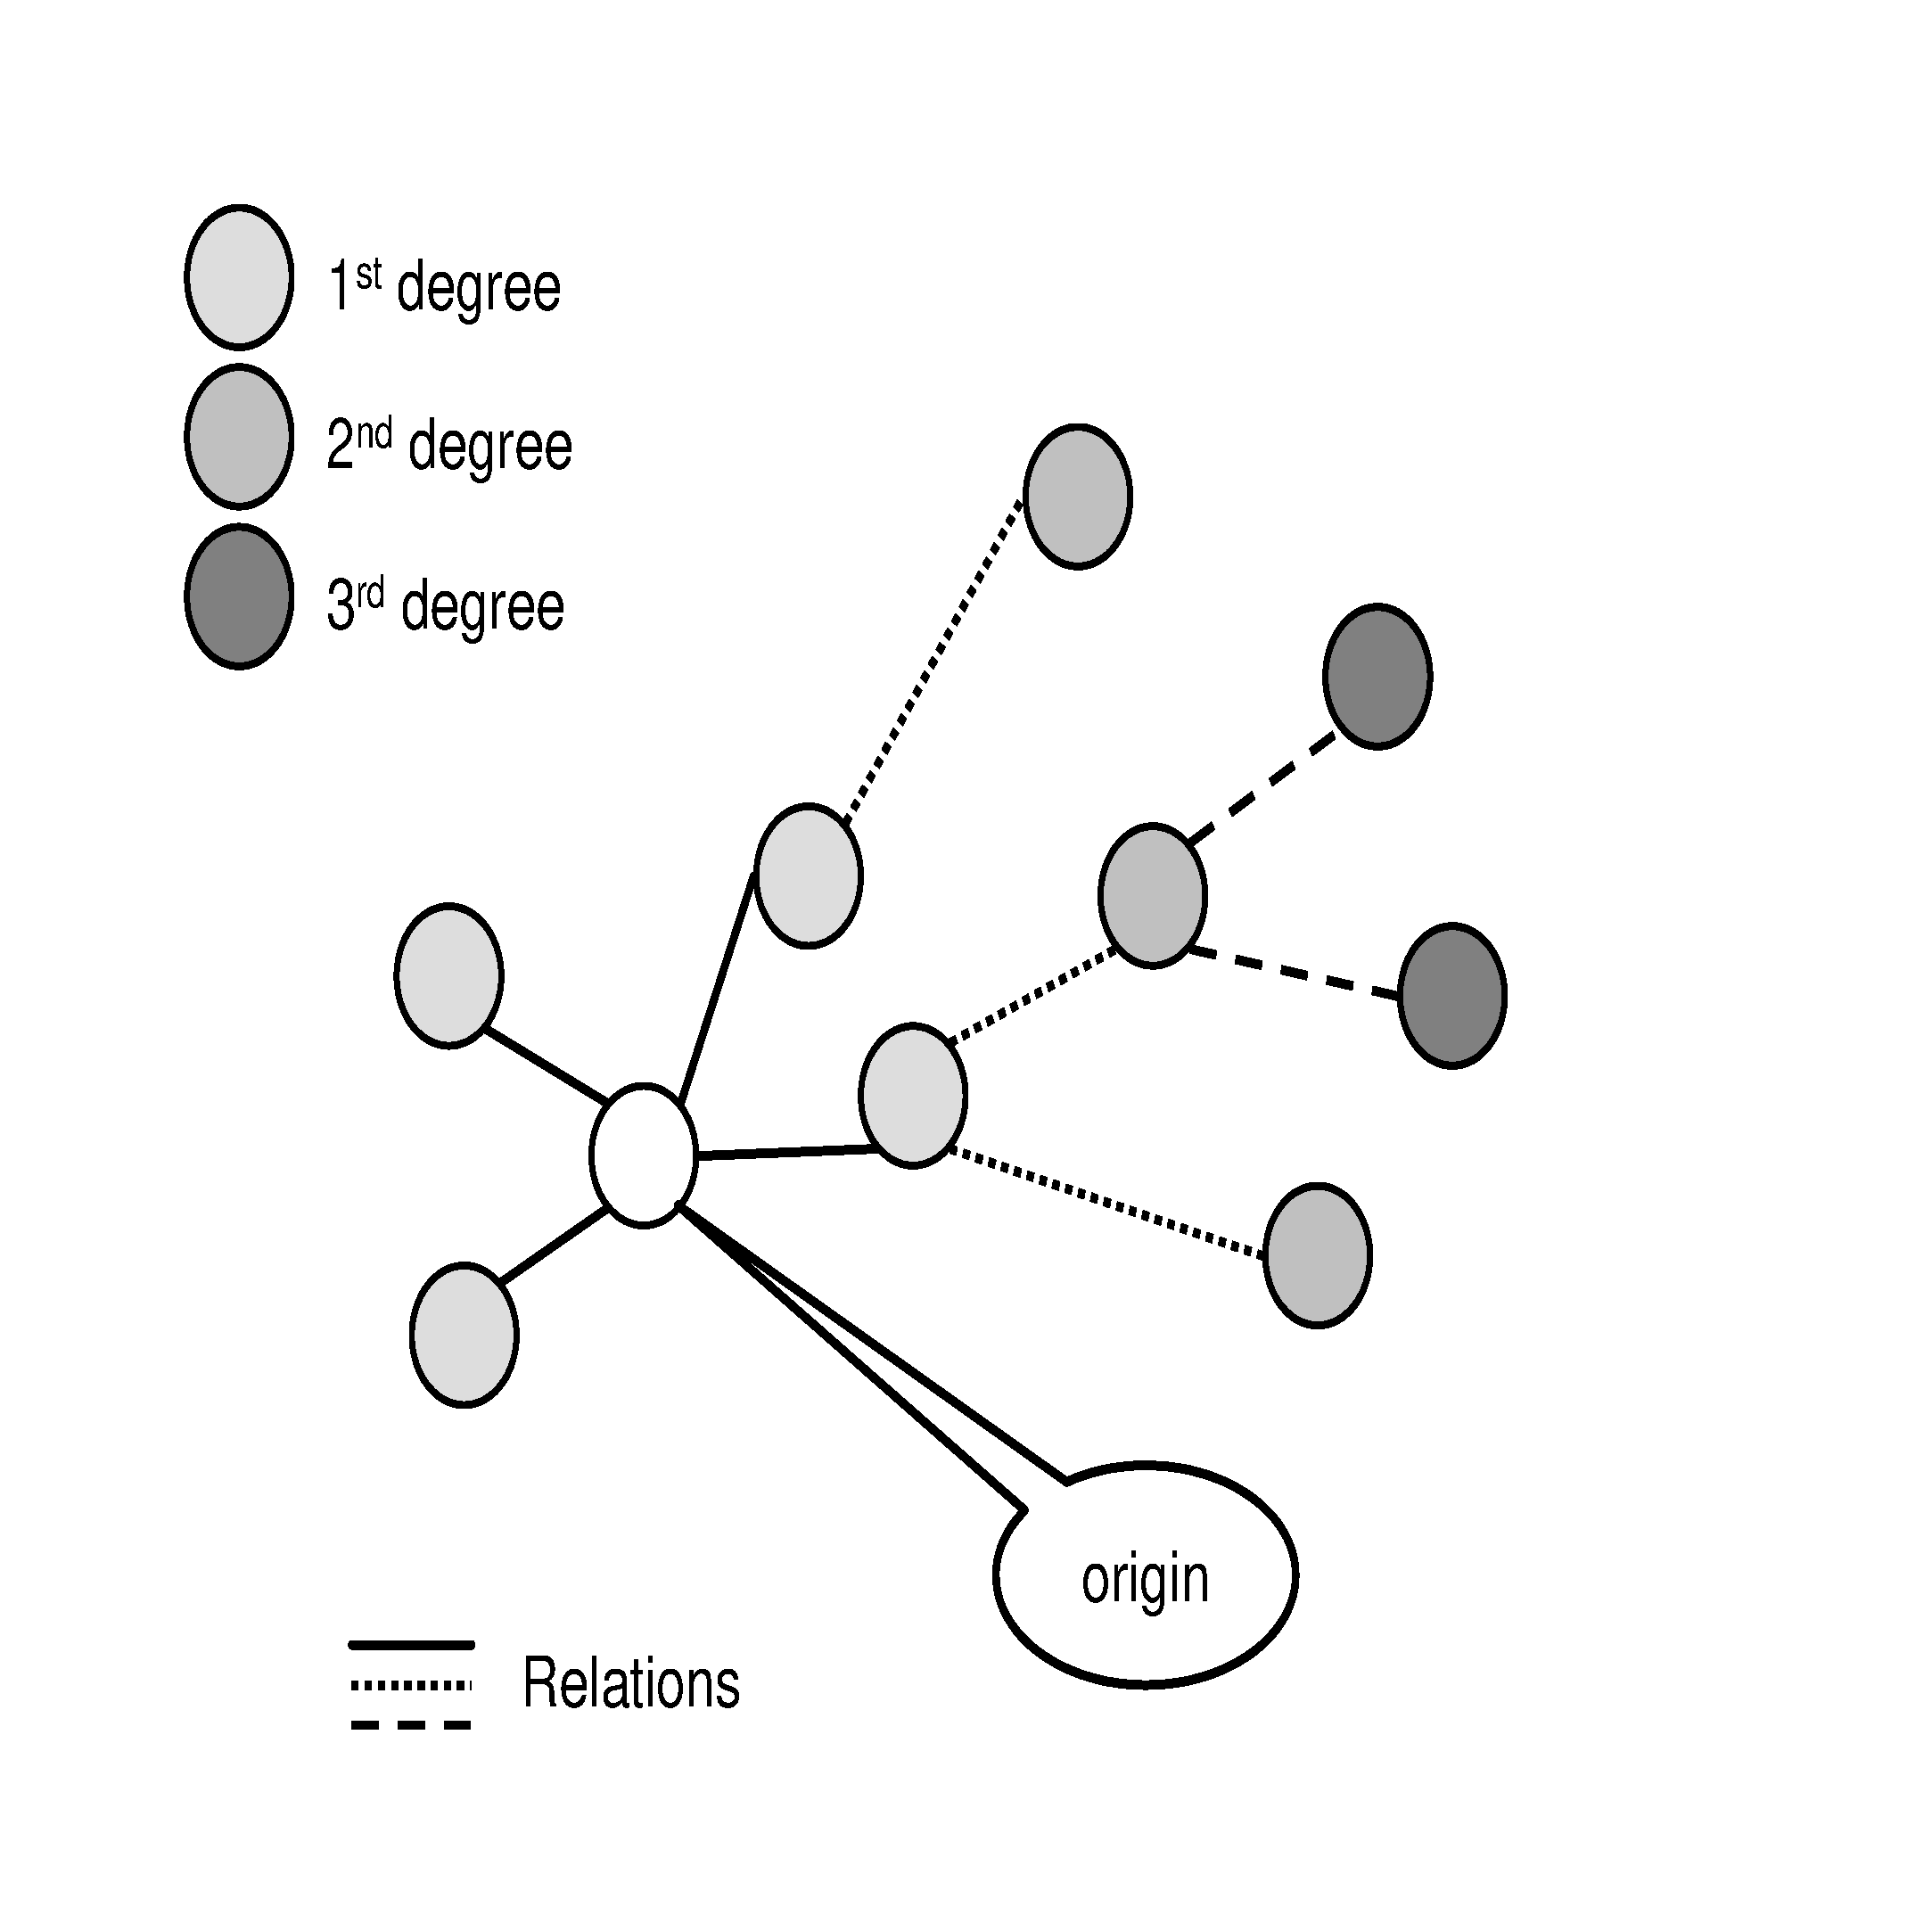
\includegraphics[width=12cm]{degrees}
	 \caption{Degrees of Relationship}
	 \label{degrees}
       \end{figure}
       The flexible setup of the relation finders means that the resulting 
       URLs may have different \textit{degrees} of relationship to the start 
       URL. 
       \begin{definition}
       If two URLs $ u_a $ and $ u_b $ are directly related by any given
       relationship $ \bullet $ (i.e. if $ u_a \bullet u_b $), 
       we call them related in the first degree.\\
       Some URL $ u_c $ is called related in the $ n^{th} $ degree to $ u_a $ if
       has no relationship with $ u_a $  but is related to an URL that 
       has a relationship of the degree $ (n-1) $ with $ u_a $. (e.g. if 
       $ u_a \bullet u_b$ and $ u_b \odot u_c $, then $ u_a $ and $ u_c $ are
       related in the second degree)
       \end{definition}
       The degree of relationship is the same as the length of a path between 
       two nodes in the graph model, and is an intuitive metric of how 
       \lq\lq far\rq\rq\ one web place is from another (Figure \ref{degrees}). 
       Since this value is very 
       useful during processing, the relation finders will mark all URLs with the 
       degree of relationship they have towards the original starting place.
     \subsection{Search Engines and Relation Finding}
       \begin{figure}[ht]
         \centering
         \includegraphics[width=12cm]{googleadv}
         \caption{Google Search Engine}
         \label{googleadv}
       \end{figure}
       Commercial web search engines like Google\cite{google} (Figure \ref{googleadv})
       or AltaVista\cite{altavista} have 
       some properties that make them well-suited for finding related URLs: They 
       use sophisticated web crawling and indexing techniques to build a 
       comprehensive index of the web, which can be queried efficiently in 
       a multitude of ways. Usually the engines not only allow simple keyword 
       searches but complex queries that can be restricted by language, 
       resource type or domain names. Some, like Google\cite{google} 
       even maintain the notion of related pages themselves, offering features like 
       \lq\lq Find related pages\rq\rq\ or \lq\lq Find similar\rq\rq . 
  
       Search engines will also use advanced ranking techniques which may be
       useful both in the DoorStep ranking phase and in selecting possible
       candidates for a relation finder heuristic.
       
       Although the algorithms and techniques used within commercial search 
       engines are often trade secrets, it can be assumed 
       that new research results are quickly adopted due to the strong 
       competition between the different engines.
       
       The main drawback of commercial search engines (besides the \lq\lq black 
       box\rq\rq\ design) is that they come with commercial terms of use. 
       Usually the
       engines may only be used freely for personal, interactive requests. An 
       example for these conditions are Google's Terms of Service\cite{googletou}:
       \begin{center}
       \begin{minipage}{10cm}
       \itshape
       [...] You may not take the
       results from a Google search and reformat and display them, or mirror
       the Google home page or results pages on your Web site. You may not
       \"meta-search\" Google. If you want to make commercial use of the Google
       Search Services, 
       [...]
       You may not send automated queries of any sort to Google's system
       without express permission in advance from Google. Note that 
       \lq\lq sending
       automated queries\rq\rq\ includes, among other things:
       \begin{itemize}
       \item{using any software which sends queries to Google to determine how
             a website or webpage \lq\lq ranks\rq\rq\ on Google for various 
             queries;}
       \item{\lq\lq meta-searching\rq\rq\ Google; and}
       \item{performing \lq\lq offline\rq\rq\ searches on Google.}
       \end{itemize}
       Please do not write to Google to request permission to 
       \lq\lq meta-search\rq\rq\
       Google for a research project, as such requests will not be granted.
       \end{minipage}
       \end{center}
       This means that publicly available DoorStep systems will have to license 
       the use of the search 
       engines\footnote{Since the inception of the DoorStep system, Google has
       a SOAP interface for automated queries.}, 
       or find free ones, if they does not want to 
       build their own web indices (which is very demanding).
     \subsection{Rating function}
       Once a set of related URLs is found, one or more 
       \textit{rating functions} will be applied to them. The goal
       of this step is to identify those web places which are the
       most interesting to the user. Since concept of \lq\lq interesting to the
       user\rq\rq\ is rather hard to describe algorithmically, we will simply 
       say that a URL (or web place) is
       interesting in some aspect $ a $ if it has certain properties that can be
       measured through a corresponding \textit{rating function} 
       $ f_a $. The rating of an URL $ u $ regarding this aspect
       can then be expressed as $ 0 \leq f_a(u) \leq 1 $.
       Examples of rating
       functions could be \lq\lq The resource does contain the specified
       keywords\rq\rq\ or \lq\lq The resource contains a text in the user's
       native language\rq\rq .
       
       The system may contain any number of rating functions $ f_1
       \dots f_n $ that measure different properties that are of interest to
       the user.
       Each of these functions has a weight
       $ 0 < \alpha_i \leq 1 $ which indicates the importance of the given 
       aspect.
       The \textit{overall rating} $ \iota $ of an URL then calculates
       to:
       \[
         \iota(u) = \sum_{i = 0}^{n} 
	 \frac{\alpha_i f_i(u)}{n}
       \]
       An rating value of 1 indicates a most interesting web place,
       while a
       value of 0 denotes a very uninteresting one. 
     \subsection{Filtering}
       The system allows for filters to be inserted between the different
       processing steps. A filter will typically check if an URL matches a
       predefined condition and discard it if it doesn't.
       
       Filtering can be used to remove \lq\lq noise\rq\rq\ from the input, to 
       speed up processing and also to remove the problem of 
       \lq\lq circular visit\rq\rq : 
       
       Would DoorStep systems be universally 
       employed, requests from one system would be registered as visits by 
       another system and the DoorStep systems would start visiting each other. 
       This can be avoided when the DoorStep system uses an unique 
       \verb$User-Agent:$ string and all visits by that agent are filtered out 
       before the processing starts.
  \section{Examples of relations}
    \label{relexample}
    In this section we will, rather than trying to do an in-depth analysis, give some 
    comprehensive examples of relations between web places and explore their 
    possible meaning. We expect that most of the relations used in the 
    DoorStep system will be taken from independent research and that the quality 
    of such relations will be extensively analysed in papers like \cite{links}.
    \\
    
    \textbf{Relation by hyperlinks:} These are probably the best understood and 
    most researched of all relations. Hyperlinks have several properties that 
    make them interesting to use in the DoorStep system: Hyperlinks are usually 
    set by people (rather than machines) and therefore denote social rather than 
    technical relations between web places. Among others, Adamic and Adar 
    showed that 
    social groups can be identified by analysing groups of hyperlinked web 
    pages\cite{links}. Hyperlinks are also very easily handle; only the original
    resource is needed to follow them and the respective relation finder does
    not need an heuristic.
    \\
    
    \textbf{Relation by domain:} DNS (sub-)domains usually denote geographic or 
    organisational groups. These can be very broad like the \verb$.com$ top 
    level domain, or quite specific like the \verb$computing.lancs.ac.uk$, 
    which is Lancaster University's computing department. 
    Finding web places within the same domain is not as 
    straightforward as following hyperlinks; the heuristic currently employed 
    in the DoorStep system is to query a commercial search engine for certain 
    keywords and restrict the search to a specific domain. This method also 
    ensures that the pages found by the relation finder are likely to be 
    of interest to the end user.
    \\
    
    \textbf{Relation by language:} Web places serving resources in the same 
    language are usually located in the same (albeit very broad) cultural background. 
    For example, a page in Japanese language is usually written by a Japanese 
    person. Additionally, the user of the DoorStep system may only understand 
    documents in certain languages and it may not be sensible to present him web 
    places that he cannot comprehend. The heuristic used for finding places with 
    a common language is the same as for finding pages in the same domain,
    except that the search is restricted to a certain language rather than to a
    specific domain.
    \\
    
    \textbf{Relation by referring search query:} As explained above, the 
    contents of the \verb$Referer:$ header (if existent) are retained within the 
    starting point URL. When a visitor was referred by a search 
    engine, the \verb$Referer:$ header will usually not only contain the 
    engine's URL, but the complete query string. This information allows a 
    relation finder to reproduce the search query and find out what other web 
    places (except our own) were returned by it. These places are related to the 
    starting URL in the way that \textit{a visitor from or from near this place was 
    potentially interested in them} and they are related to our own place in
    that they show up in the result of the same search query.
    \\
    
    \textbf{Relations from search engines:} Web search engines often maintain 
    their own notion of \lq\lq related\rq\rq\ pages, like Google's 
    \lq\lq Find related\rq\rq\ feature. While the exact definition of those 
    relations is hidden within the search engine, a relation finder can 
    easily exploit them by sending a search query.
    \\
    
    \textbf{Relation by similar hostname:} Some researchers (like 
    \cite[Link Affiliation]{experts}) 
    treat web places with similar host names as related. For example they 
    assume that hostnames with the same prefix (like \verb$www.apple.com$ and
    \verb$www.apple.co.uk$) belong to the same organisation. A heuristic for 
    finding this kind of relation could be somewhat more complicated since most 
    commercial search engines lack the appropriate query options.
    \\
    
    For those heuristics that employ the use of search engines, it is important 
    to carefully select the search keywords. While the simplest method is to use 
    a set of static keywords, which are deemed to be interesting to the user, 
    more sophisticated algorithms could also select new keywords from the web 
    places that have already been found.
  \section{Examples of rating functions}
    \label{rateexample}
    Many different approaches to the problem of ranking web pages, 
    like PageRank\cite{page}, Topic Distillation\cite{kleinberg} or
    anchor-text analysis\cite{chakrabarti} have been proposed by the research
    community. Although we expect those algorithms to perform well, they are
    usually quite complex and not always easy to implement.
    Many, like the popular Link Rating\cite{page}\cite{kleinberg}
    even require a more or less comprehensive web index, something that is difficult 
    to build and maintain within a research project. For this reason, we will not 
    discuss those functions here, and instead present some simpler, home-grown 
    ones which are easy to implement and should perform reasonably well 
    within the DoorStep system. Nonetheless, it is always possible to enhance 
    the system with some more advanced rating functions, if desired.
  
    \textbf{Keywords matching META tags:} This function can be used if the
    resource served by an URL is a HTML document containing tags of the form
    \verb$<meta name="keywords" content="keyword1,keyword2,..." />$ 
    We assume that the user's interest is expressed in a list of $ n $ keywords,
    and for each occurrence of one of those keywords in the \verb$meta$
    keyword list $ KL $ the rating will be increased by $ 1/n $. Thus
    the rating will calculate to:
    \[
      f_{\mbox{meta}}(u) = \sum{k_i \in KL_u} \frac{1}{n}
    \]
    \\
    
    \textbf{Keywords matching document body:} Especially if the page does not
    contain any \verb$meta$ tags, we can try to find the keywords in the
    document's body. Since a word may occur in a page more than once, we should
    also take the number of occurrences in account. ($ n(k_i) $ is the number of
    occurrences of the keyword $ k_i $).
    
    We will use a weight function $ w $ that assigns a weight to the occurrences
    of each keyword so that $ 0 \leq w(n(k_i)) \leq 1 $ and calculate the
    rating of the URL to
    \[
      f_{\mbox{key}}(u) = \sum_{k_i \in u} \frac{w(n(k_i))}{n}
    \]
    In the testbed implementation we then used a logarithmic function for 
    $w()$ that will quickly increase with the first few occurrences of a 
    keyword, but raise the rating more slowly if a huge number of occurrences is 
    involved:
    \[
      w_1(n) = - \frac{1}{log((n - \alpha) \beta) + 1}
    \]
    \[
      w(n) = \left\{
      \stackrel{w_1(n) \hspace{2mm} | \hspace{3mm} 0 \leq w_1(n) \leq 1}
      {0 \hspace{3mm} \mbox{otherwise}}
      \right.
    \]
    The parameters $ \alpha $ and $ \beta $ control the behaviour of the
    logarithmic function: While $ \alpha $ controls the \lq\lq threshold\rq\rq\
    (the number of occurrences needed to get a rating $ \geq $ 0), $ \beta $
    controls how quick the rating grows when new occurrences are found. For the
    test system we used $ \alpha = 2 $ and $ \beta = 1 $.
    \\
    
    \textbf{Note on keyword matching functions:} While the methods above worked
    well in tests, they had problems in the more extensive trials. These
    problems (which will be explained in detail with the other test results)
    were not necessarily caused by the simplicity of the functions, they were
    due to the fact that describing the user's interest as a list of keywords is
    a very limited view.
    \\
    
    \textbf{Language or Domain match:} When one assumes that pages in a specific 
    language, within a specific domain or with some other static property are 
    more interesting to the user than others, a rating function can assign a 
    fixed rating to those pages.
    \\
    
    \textbf{Use search engine rating:} Most commercial search engines employ a 
    number of advance rating techniques. Although those mechanisms are 
    usually kept secret and cannot be accessed directly, they are reflected in 
    the results of the search queries. A rating function can exploit this property 
    and assign a higher rating to pages that show up at the top of the search 
    results than to those on the bottom.
  \section{Test Implementation}
      In order to evaluate our assumptions, we implemented a testbed that 
      allowed us to test the DoorStep system in a real-life environment, using 
      the relations and rating functions given in Sections \ref{relexample} and
      \ref{rateexample}.
    \subsection{Testbed Architecture}
      The testbed consists of a collection of modules, exchanging XML formatted 
      data: There is one XML format to describe generic \textit{visit events} 
      (Figure \ref{visitxml}) and another to describe \textit{web 
      places} (i.e. URLs, Figure \ref{urlxml}). Each module will read XML 
      documents of one of those formats and will produce a document in the URL 
      description format as an output.
      
      \begin{figure}[ht]
        \centering
        \includegraphics[width=12cm]{gilbert_steps}
        \caption{Setup of the modules}
        \label{gilbert_steps}
      \end{figure}
      \begin{figure}[ht]
\begin{verbatim}
<visitlist>
  <visit>
    <type>Html</type>
    <timestamp>01:11:2001:00:00:42</timestamp>
    <visitor>
      <class>remote</class>
      <class>agent</class>
    </visitor>
    <resource>/lehre/ubiq/kontext/html/tsld010.htm</resource>
    <host>dudley.waltham.northernlight.com</host>
    <location_code>244</location_code>
  </visit>
  <!-- The file may contain more visits -->
</visitlist>
\end{verbatim}
        \caption{XML format for visits}
	\label{visitxml}
      \end{figure}
      \begin{figure}[ht]
\begin{verbatim}
<url_list>
<url>
  <name>http://dudley.waltham.northernlight.com/</name>
  <location_code>244</location_code>
  <timestamp>01:11:2001:00:00:42</timestamp>
  <degree>0</degree>
  <interest>0.5344394</interest>
  </url>
  <!-- The file may contain more URLs -->
</url_list>
\end{verbatim}
        \caption{XML format for URLs (web places)}
	\label{urlxml}
      \end{figure}
      
      The modules are arranged in a daisy-chain (Figure \ref{gilbert_steps}), 
      with a visit-to-url module 
      (called an \textit{extractor}) at the head of the chain and any number of 
      url-to-url modules (called \textit{refiners}) following. 
      
      The contract of 
      an extractor module requires that it finds URLs close to the visits given 
      in the input document (thus performing the first step in the DoorStep 
      processing chain). The \textit{extractor's} output is expected to be a 
      document describing those URLs. 
      
      The contract of a \textit{refiner} module 
      demands that it acts either as a \textit{relation finder} or a 
      \textit{rating function}. If the \textit{refiner} implements a rating 
      function, it is expected to assign a rating value to each of the URLs on 
      the input. If an URL already has a rating, it shall be modified according 
      to the \textit{refiner's} internal weight. A \textit{refiner} acting as a 
      \textit{relation} finder is expected to read the URLs from the input 
      document and find other places related to them (by a relation that is 
      configured within the \textit{refiner} module).
      
      A \textit{refiner} that is a \textit{relation finder} can be configured 
      to have a maximum degree of relationship. If a URL's degree of
      relationship towards the starting point is higher than this
      value, the relation finder will \emph{not} attempt to find
      any more relatives. In the graph model this is equivalent to the relation
      finder ignoring all vertices that do not have a know path to the starting
      point that is shorter than $ x $  (where $ x $ is the maximum degree of
      relationship).
      
      The maximum degree of relationship allows refiners to mimic the flexible 
      setup shown in 
      Figure \ref{relations}, while only being
      connected in a daisy-chain. (\textit{Refiners} acting as rating 
      functions must ignore the degrees of relationship. It is also required 
      that rating functions must be on the end of the chain.)
      
      Finally, each module (refiner or extractor) in the system can contain one
      or more 
      filters. A filter may drop any entity (visit or URL) before it enters the
      module, causing the dropped entity to be removed from all further
      processing.
    \subsection{Test Framework}
      For practical reasons we created a framework of Java classes that 
      implements the basic functionality of the \textit{extractors} and 
      \textit{refiners}, is capable of handling the connections between the 
      modules and takes care of recurring tasks (e.g. XML decoding or search 
      engine requests). Within this framework a new module type can (in many 
      cases) be implemented simply by overwriting a single method of the 
      framework's superclass.
      
      Nevertheless it is not required that each module is part of the 
      framework, or even written in Java at all. As long as a module is able to 
      understand the respective XML format(s), and conforms to the contracts 
      given in the previous section, it should be able to interact with all 
      other modules.
    \subsection{User Display}
      The testbed also contains a display architecture that shows a \lq\lq slide
      show\rq\rq of the resulting web pages. The architecture consists of a
      Java-driven web application using servlets and JSPs and requires only a
      standard web browser as a front end (Figure \ref{javaclient}. 
      Alternatively, the Display may run as
      a small VisualBasic application\footnote{Written
      by Albrecht Schmidt} that is directly driven by a Java server
      process and offers some additional functionality (Figure \ref{vbclient}.
      
      The display is meant to run on a separate screen in the user's environment
      and change infrequently (i.e. every 2 to 10 minutes) to a new web place.
      If the user is interested in a certain page he has the option to stop the
      slide show and explore that page further (by following the hyperlinks). 
      The slide show will automatically commence after a while.
      \begin{figure}[ht]
       \centering
	 \includegraphics[width=12cm]{javaclient}
	 \caption{Java Based Display}
	 \label{javaclient}
       \end{figure}
      \begin{figure}[ht]
        \centering
        \includegraphics[width=12cm]{vbclient}
        \caption{Visual Basic Based Display}
        \label{vbclient}
      \end{figure}
      
      For a first user study, we plan to use this software on a panel computer 
      that can easily be fitted into the user's surroundings (Figure \ref{ppc}. 
      The machine is 
      equipped with a touch-sensitive panel for intuitive user interaction and 
      should easily blend into any office environment. This kind of ambient 
      display should be unobtrusive to the user while, at the same time, enabling 
      him to check his web surroundings whenever he chooses to.
      \begin{figure}[ht]
        \centering
        \includegraphics[width=12cm]{ppc}
        \caption{Panel PC used for Display}
        \label{ppc}
      \end{figure}
  \section{Walk-Trough Scenario}
    In this small scenario we will follow the way that three visit events take    
    through the system. We will see how the visits are handled and how related 
    web places are found. Our example system will be set up in the following 
    way (line numbers given for reference only):
    \begin{verbatim}
010 extractor = new ExtractingChain(dataSource);
020 String keywords = "wearable,ubicomp";
030  
040 Extractor ext = new StraightExtractor();
050 ext.addPrefilter(new LocalVisitFilter());
060 ext.addPrefilter(new AgentVisitFilter());
070 extractor.setExtractor(ext);
080        
090 SearchingRefiner search = new SearchingRefiner();
100 search.setKeywords(keywords);
110 extractor.addRefiner(search);
120        
130 extractor.addRefiner(new LinkRefiner());
140                
150 KWInterestRefiner kwr = new KWInterestRefiner(); 
160 kwr.setKeywords(keywords); 
170 extractor.addRefiner(mkr); 
      \end{verbatim} 
      
      The \verb$ExtractingChain$ in line 10 is an utility object that will 
      connect the Extractor and several refiners. The \verb$StraightExtractor$ 
      in line 40 implements the algorithm introduced in section
      \ref{findstart}, and 
      it's prefilters (lines 50 and 60) will discard visits that come from the 
      local network, or any automated web agent (the local network for this
      example is \verb$lancs.ac.uk$).
      
      The \verb$SearchingRefiner$ in line 90 will search for URLs in the same 
      domain as the starting point and the \verb$LinkRefiner$ (line 130) will 
      follow hyperlinks.
      
      Finally, the \verb$KWInterestRefiner$ in Line 150 will use the rating 
      function introduced in \ref{rateexample} to rate the URLs.
    \subsection*{Starting up}
      The visits recorded in the web servers log file will probably read
      like this (lines have been abbreviated):
      \begin{verbatim}
dyn007.dhcp.lancs.ac.uk [30/Nov/2001:17:00:45] "GET /~kristof"
teco88mc.teco.uni-karlsruhe.de [30/Nov/2001:17:04:33] "GET /~kristof"
cw01.dd1.srv.t-online.de [30/Nov/2001:17:19:12] "GET /~kristof"
      \end{verbatim}
      The first visit is from our local network (\verb$lancs.ac.uk$), the
      second comes from a research institution (the TeCo in Karlsruhe) and the
      third is a visitor from a big commercial service provider (T-Online in
      Germany).
      
      Before the actual processing starts, the log file is read by a small
      script that converts it into an XML file readable by the toolkit:
      \begin{verbatim}
<visitlist>
  <visit>
    <type>Html</type>
    <timestamp>30:11:2001:17:00:45</timestamp>
    <visitor>
      <class>person</class>
      <class>local</class>
    </visitor>
    <resource>~kristof/</resource>
    <host>dyn007.dhcp.lancs.ac.uk</host>
    <location_code>223</location_code>
  <visit>
  <visit>
    ...
    <visitor>
      <class>remote</class>
      ...
    </visitor>
    <host>teco88mc.teco.uni-karlsruhe.de</host>
    ...
  </visit>
  <visit>
    ...
    <visitor>
      <class>remote</class>
      ...
    </visitor>
    <host>cw.dd1.srv.t-online.de</host>
    ...
  </visit>
</visitlist>
      \end{verbatim}
      In the XML file, each \verb$<visit>$ entry corresponds to one line of the
      log file, and most of the tags contain one of the log file's data fields
      (the XML may contain additional fields, e.g. for \verb$Referer:$ or 
      \verb$User-Agent:$ information). The \verb$<visitor>$ tag already
      contains some classification of the visit: It indicates if the visit came
      from the local network (\textit{local} or \textit{remote}) and whether the
      visitor was more likely a real person or an automated web agent. The
      \verb$<type>$ tag indicates the type of the visit, and is to be used in
      further extensions.
    \subsection{Starting Point Extraction}
      The \verb$StraightExtractor$ will now read the visits from the XML file,
      passing each visit through it's internal filters before processing. The
      first visit is dropped by the \verb$LocalVisitFilter$, since it comes
      from our own network. The other two visits pass and the extractor
      attempts to find \textit{living} start URLs, using the algorithm from
      Section \ref{startingsection}. The possible starting URLs will be checked in the
      order:
      \begin{itemize}
        \item{\verb$teco88mc.teco.uni-karlsruhe.de$}
        \begin{itemize}
          \item{\verb$teco88mc.teco.uni-karlsruhe.de$ (not alive)}
          \item{\verb$www.teco.uni-karlsruhe.de$ (alive)}
          \item{\verb$www.uni-karlsruhe.de$ (alive)}
        \end{itemize}
        \item{\verb$cw.dd1.srv.t-online.de$}
        \begin{itemize}
          \item{\verb$cw.dd1.srv.t-online.de$ (not alive)}
          \item{\verb$www.dd1.srv.t-online.de$ (not alive)}
          \item{\verb$www.srv.t-online.de$ (not alive)}
          \item{\verb$www.t-online.de$ (alive)}
        \end{itemize}
      \end{itemize}
      As we can see, the algorithm works well on the research visitor, finding
      both the research institute's homepage and the university homepage. For
      the ISP visitor, on the other hand, the algorithm only finds the ISP's
      homepage (Figure \ref{tolhome}.
      
      \begin{figure}[ht]
        \centering
        \includegraphics[width=12cm]{tolhome}
        \caption{ISP Portal (T-Online)}
        \label{tolhome}
      \end{figure}
      
      The extractor will then encode it's results in XML again (abridged):
      \begin{verbatim}
<url_list>
  <url> 
    <name>http://www.teco.uni-karslruhe.de/</name> 
    <location_code>54</location_code> 
    <timestamp>30:11:2001:17:00:45</timestamp> 
    <degree>0</degree> 
  </url> 
  <!-- Other URLs from example not shown here --> 
</url_list>
      \end{verbatim}
      Since the URLs in this file are the descriptions of the starting places,
      they have a degree (of relationship) of 0. Had the original visit
      contained
      \verb$Referer:$  fields or similar information, this would also have been
      preserved in the corresponding \verb$<url>$ tags.
    \subsection{Searching the domain}
      The starting points will now be fed into the \verb$SearchingRefiner$,
      which will look for other web places in the same DNS domain. For this, the
      refiner will query a search engine, using the pre-configured keywords and
      restricting the search to the domain of the starting place. The current
      implementation of the refiner is very simple; it will always use the two
      rightmost tokens of the host name as the domain. 
      
      
      
      \begin{figure}[ht]
        \centering
        \includegraphics[width=12cm]{ubicompag}
        \caption{Research Home Page (Rated High)}
        \label{ubicompag}
      \end{figure}
      
      With this method the refiner in our example will (for the first URL)
      create a query that is equivalent to \lq\lq Search the domain
      \verb$uni-karlsruhe.de$ with the keywords ubicomp and wearable\rq\rq .
      This search will return several ubicomp-related pages at the University of
      Karlsruhe, including the homepage of the ubicomp student group at 
      \textit{http://www.uni-karlsruhe.de/AG-Ubicomp.htm} (Figure
      \ref{ubicompag}, the URL
      was changed for better readability). The refiner will parse the search
      results and encode them into XML (abridged):
      \begin{verbatim}
<url_list>
  <url> 
    <name>http://www.teco.uni-karslruhe.de/</name> 
    <location_code>54</location_code> 
    <timestamp>30:11:2001:17:00:45</timestamp> 
    <degree>0</degree> 
  </url> 
  <url>
    <name>http://www.uni-karlsruhe.de/AG-Ubicomp.htm</name> 
    <timestamp>30:11:2001:17:00:45</timestamp> 
    <degree>1</degree> 
  </url>
  <!-- Other URLs not shown in example --> 
</url_list>
      \end{verbatim}
      
      We see that the newly found URLs have a degree of relationship of 1
      towards the original starting places and that the original starting places
      are also in the refiner's output. The latter is done by most refiners -- no
      matter what relation they work on -- in order not to loose interesting web
      places. If this behaviour is not desired, the refiner may either allow the
      user to disable it during runtime or disable it permanently.
      
      When we look at the results of the two searches 
      (one in the \verb$uni-karlsruhe.de$ domain and one in \verb$t-online.de$),
      we see that the search in the university's domain found many
      research-related documents while on T-Online we discovered commercial pages
      with product reviews and the like. This behaviour is expected and desired: 
      Each kind
      of pages reflects a different online \lq\lq territory\rq\rq\ from which
      the visitor came.
    \subsection{Following the links}
      The next refiner in the chain is the \verb$LinkRefiner$. It will attempt
      to read the resources of all the URLs in the input file and, if the
      resources are HTML pages, follow the hyperlinks contained in them.
      
      For example, when the refiner encounters the ubicomp group's homepage, it
      will find links to the professors, the home page of the corresponding
      lecture, to researchers whose work will be presented and to other groups.
      The T-Online product review pages contain links to in-depth articles,
      photo collections, small movies and to the manufacturer of the products
      (Figure \ref{xyberhome}).
      
      A unresolved problem with both kinds of pages is that the \lq\lq
      framework\rq\rq\ of the page (i.e. the navigation bars) contain very
      generic hyperlinks that are neither necessarily related to the page's content
      no especially useful for the system.
      Nevertheless, following hyperlinks is quite effective, and one of the
      researchers linked on an institute's homepage may even be the virtual home
      of the original visitor.
    \subsection{Rating and Display}
      All URLs will finally be passed through the \verb$KWInterestRefiner$
      which
      calculates a rating for each of them. The rating will be written back
      to the XML in an \verb$<interest>$ tag:
      
      \begin{verbatim}
...
<url>
  <name>http://www.uni-karlsruhe.de/AG-Ubicomp.htm</name> 
  <timestamp>30:11:2001:17:00:45</timestamp> 
  <interest>0.2134538</interest>
  <degree>1</degree> 
</url>
...
      \end{verbatim}
      
      Although the rating function works reasonably well for some pages, it has
      one major drawback: Web Places can be interesting to the user although
      they aren't directly related to the keywords of the rating function and
      many places that are found by other means than a web search receive
      a rating of 0. While the best way to address this problem is to implement
      better and more adaptive rating functions, we currently work around it by
      introducing an amount of randomisation into the display routine. 
 
      \begin{figure}[ht]
        \centering
        \includegraphics[width=12cm]{xyberhome}
        \caption{Manufacturer Page (linked from ISP, rated zero)}
        \label{xyberhome}
      \end{figure}
      Pages with high
      ratings are preferred by the system but pages with inferior ratings will
      still be shown. In this way the user will not only get information
      directly related to the predefined topics, but also pages like those of
      manufacturers that have related products.
  \section{Test System Performance} 
    Although a formal user study has yet to be planned, we did 
    preliminary tests on the system in two ways: First we installed the JSP 
    server (with a setup similar to that in the walk-through example) 
    on a machine available to the research group, and fed it with the 
    log data from our own web server (at 
    \textit{http://ubicomp.lancs.ac.uk/)}. This allowed us not only to test 
    the long-term stability of the software, but also to observe if and how 
    the system would be used. In many cases we were quite surprised about 
    the web places found by the system, and most of them were related to our 
    research. The main problem with the test setup was that the traffic on 
    our own machine is quite low, allowing the system to find new places 
    only very infrequently which in turn resulted in a very repetitious 
    \lq\lq slide show\rq\rq .
    
    Researchers that did not have their own display 
    for the DoorStep system did not use it permanently, but rather looked 
    the page up during their spare time.
    
    For the second test, we performed some offline processing on a large log 
    file, in order to get some statistical results. This test will be explained 
    in detail in the next section.
    \subsection{Test Data}
      The test dataset is part of the HTTP log file from a research lab
      web server. The log file contains about 200.000 entries from a period of
      about 2 weeks.
      
      The file contains a high amount of redundancy and noise: The 200.000 
      entries record visits from only 5720 different clients. Of those, 1603 
      were either visits from local clients (within the same network as the 
      server), failed to retrieve a resource or were requests for pictures 
      within sites.
      
      Most of the original request (of those that did not fail) (82\%) came from a 
      machines with a proper
      DNS host name, and only 18\% from unresolveable addresses -- this indicates
      that methods requiring qualified DNS names should work reasonably well. A
      substantial amount of the entries also carried additional information:
      Almost 40\% of the requests were made by automated agents (e.g. web
      crawlers) that idendentifiable by an \verb$User-Agent$ String and 8\% of
      were referred to the site as the result of a web search (with the search
      string showing up in the \verb$Referer$ field). 
    \subsection{Results}
      For the trials we used almost the same refiners and extractor as in the
      walk-through example, although in different setups. The input to the 
      system consisted of the 3500 unique and successful visits from the original 
      log. 
      
      From the original visits, 
      the \textit{extractor} module found about 1500 URLs that
      were \textit{alive}. This is a reasonably good set of starting places,
      however a first look at the data revealed that most of them were either
      ISP portal pages or homepages of academic institutions. While the latter
      are in most cases good starting points for further processing, ISP portal
      are rather unspecific and uninteresting in the context of this system.
      This behaviour is mostly due to the fact that many of the \lq\lq
      mundane\rq\rq\ (i.e. non-academic) visitors are \lq\lq homeless\rq\rq\ in
      the sense that the do not have their own web place -- and even if they do
      they often enter the web from a place that is far removed from their own
      place. In a purely academic setting (like ours) this problem is less
      pressing since the user's home place (or -page) is usually located within
      the same network from which the user enters the web. This \lq\lq homeless
      visitor problem\rq\rq\ has already been observed in \cite{webaware};
      this will be an issue for further research.
      
      It showed that the web searched based approach was much more selective
      than following the hyperlinks: The 1500 original URLs grew to only about 
      4000
      with the web search approach, but to almost 39000 in when we followed the
      hyperlinks. When we used the searching module on these URLs, we gained
      only an additional 1000, coming to a total of 40000. If this result is
      correct it would mean that the collection of linked contains almost all
      pages that are found by the web search. On the other hand, following the
      links from those pages that were originally found by the search heuristic
      was very productive: From 4000 original URLs we got almost 86000 places on
      the output.
      
      With the rating function we observed an obvious problem: Although, as
      expected, the pages found by the search heuristic got positive results
      (i.e. ratings $ > 0 $) virtually all of the original places and those
      found by following hyperlinks got a rating of 0. Since we assume that many
      of those places are interesting to the user we conclude that a keyword
      list (at least in it's current form) is not a very good model of the
      user's interests. While we are of the opinion that a high rating by the
      current function \emph{does} denote an interesting place, many of those
      URLs rated with 0 will also be interesting in some other regard.
      Therefore, to improve the quality of the rating, it will be necessary to
      do further research into user's interests and how they can be measured.
      
      It is likely that even the more advanced rating functions from the
      literature will reveal the same problem, since they were designed the
      measure pages against a search query, not against an abstract \lq\lq
      interest of the user\rq\rq .
  \section{Privacy: Reassuring the Visitors}
    A system that, like DoorStep, collects and analyses user data must always 
    take privacy considerations into account. 
    
    In practice, usage data falls into two broad categories: Statistical usage 
    data which cannot be linked to any particular user, and is therefore less 
    confidential, and personal data which identifies the 
    person to which it \lq\lq belongs\rq\rq . The personal data is 
    sometimes further divided according to confidentiality: While the address or 
    phone number of a person is usually publicly known, medical records should 
    be kept strictly confidential. 
    
    It is generally agreed that it is the 
    responsibility of the operator of any data processing service to safeguard 
    sensitive personal data, although there are disagreements on how this should
    be achieved.
    
    Due to technical and legal requirements a lot of sensitive personal 
    information is stored within web server log files; each request will be 
    logged on all machines along it's way. If the log information is 
    combined, it is not only possible to link each page view to a particular 
    person but also to create a profile of that person's behaviour on the web. 
    And although the extent of logging is by no means a secret, the majority 
    of web users are unaware of it, perceiving the web as a place of anonymity.
    The latter is true even for those who know about the web server logs because
    they simply assume that the information there will probably never be read.
    
    The use of sensitive information, like that contained in web server logs,
    is tightly regulated in many parts of the world. Despite the fact 
    that some countries (like the USA) leave privacy considerations largely to 
    the forces of the market, others have imposed a rather strict legislation: 
    In Germany, for example, even legally collected personal information may 
    only be used for purposes to which the \lq\lq owner\rq\rq\ has previously
    agreed. 
    
    Luckily for the DoorStep system it does not collect additional personal
    information, and all the information that it displays is public 
    (the web pages that are displayed by the system can hardly be 
    regarded as confidential). While the legal implications of this
    constellation can be further researched, we believe that the DoorStep system
    may be legally employed in most places -- especially if the visitors are
    notified about the fact. The latter will also introduce an element of
    transparency:  Even though most users are quite oblivious of privacy 
    considerations in areas they feel \lq\lq safe\rq\rq\ in, they often are very 
    careful about new developments (e.g. student's comments about the current 
    project ranged from \lq\lq doggy ground\rq\rq\ to \lq\lq Big Brother\rq\rq 
    ).
    
    Engineers are often surprisingly aware of the privacy implications of their 
    inventions, and many specification documents warn against the abuse of 
    certain features -- like, for example, the HTTP specification\cite{http}:
    
    \begin{center}
       \begin{minipage}{10cm}
       \itshape
          A server is in the position to save personal data about a user's
          requests which might identify their reading patterns or subjects of
          interest. This information is clearly confidential in nature and its
          handling can be constrained by law in certain countries. People using
          the HTTP protocol to provide data are responsible for ensuring that
          such material is not distributed without the permission of any
          individuals that are identifiable by the published results.
   
          [...]
   
          The Referer header allows reading patterns to be studied and reverse
          links drawn. Although it can be very useful, its power can be abused
          if user details are not separated from the information contained in
          the Referer. Even when the personal information has been removed, the
          Referer header might indicate a private document's URI whose
          publication would be inappropriate.
       \end{minipage}
    \end{center}
    
    If the DoorStep (or a similar) system sees widespread use, the safest and 
    most transparent thing to do would be to include an option into the
    visitor's user agent that allows him to have his visits excluded from the
    DoorStep processing. Visitors may also attempt to obscure their origin by
    using publicly available \lq\lq anonimizer\rq\rq\ services, and the DoorStep
    system should exclude visits by those services from processing.
  \section{Conclusions and Further Work} In this work we showed that, using 
    the notion of \textit{relations} between web places, it is possible to build 
    a system that can help to visualise the connections between a site and the 
    visitors. The system should renew the hosts' interest in maintaining his own 
    web place and, by allowing a look into the virtual surroundings, give new 
    incentives for improvements. The test installation has been well received 
    within the group, and the results were interesting and surprising. On one 
    occasion a researcher even messaged us if we could \lq\lq wind back\rq\rq\ 
    the slide show to an interesting page that he saw -- this feature will be 
    implemented in a future version.
    
    For interested users we may also keep a public DoorStep web server running
    so that everyone with a spare machine will be able to use the system.
    
    Initial user reactions within the research group were positive and we now
    plan to conduct a small user study that will allow us to study users
    reactions over the period of a few weeks. We hope to get an impression on how
    the use of the DoorStep system changes the host's attitude towards his own
    web place and which places he will be most interested in. The results of the
    user study will also go into the future development of the system.
    
    In the future we plan to make the DoorStep system more adaptive,
    rather than relying on a fixed set of keywords it will learn the user's
    preferences and modify it's behaviour in different environments. This
    adaptiveness we be especially needed in the rating functions which, in their
    current form, show serious weaknesses.
    
    We also need
    to fix the \lq\lq homeless visitor problem\rq\rq : The most permanent
    solution would be for the visitor to supply his own home URL \cite{webaware},
    through an additional HTTP header field, although this would require
    modifications to the visitor's client software. Other options would include
    to use information from existing profiling systems or
    information from user accounts.
  \newpage    
  \begin{thebibliography}{99}
    \bibitem{awstats} AWStats Tool
    \bibitem{webaware} Hans-W. Gellersen and Albrecht Schmidt.
    Look who's visiting: supporting visitor awareness in the web.
    Academic Press, 2000.
    \bibitem{experts} Krishna Bharat and George A. Mihaila.
     When Experts Agree: Using Non-Affiliated Experts to Rank Popular Topics,
     Proceedings of the WWW10 Conference, 2001.
     http://www10.org
    \bibitem{flake} C. Flake, S. Lawrence and C. Lee Giles.
    Efficient identification of web communities.
    Sixth ACM SIGKDD International Conference on Knowledge Discovery and Data 
    Mining, Boston, MA, 2000. 
    pp. 150-160
    \bibitem{gibson} D. Gibson, J. Kleinberg and P. Raghavan.
    Inferring Web communities from link topology.
    Proceedings of the 9th ACM Conference on Hypertext and Hypermedia, 1998.
    \bibitem{links} Lada A. Adamic and Eytan Adar.
    Your are what you link, Proceedings of the WWW10 Conference, 2001.
    http://www10.org/program/yawyl/YouAreWhatYouLink.html
    \bibitem{larson} R. R. Larson.
    Bibliometrics of the World Wide Web: an exploratory analysis of the
    intellectual structure of cyberspace.
    Global Complexity: Information, Chaos and Control, Annual Meeting of the
    American Society for Information Science, 1996.
    \bibitem{page} S. Brin and L. Page.
    The anatomy of a large-scale hypertextual web search engine, 
    Proceedings of the WWW10 Conference, 2001.
    http://www10.org
    \bibitem{kleinberg} J. Kleinberg.
    Authoritative sources in a hyperlinked environment, Proceedings of the WWW10
    Conference, 2001.
    http://www10.org/
    \bibitem{chakrabarti} S. Chakrabarti, B. Dom et. al.
    Experiments in topic distillation.
    Proceedings of ACM SIGIR Workshop on Hypertext Information Retrieval on
    the Web, 1998.
    \bibitem{ambient} Hans-W. Gellersen, Albrecht Schmidt and Michael Beigl.
    Ambient Media for Peripheral Information Display.
    \bibitem{windows} Liechti O, Siefer N and Ichikawa T.
    A non-obtrusive User Interface for Increasing Social Awareness on the 
    World Wide Web. Personale Technologies 3 (1\&2), 1999.
    \bibitem{url} RFC 1738. Uniform Resource Locators (URL) 
    \bibitem{logfile} Log file RFC.
    \bibitem{google} Google search engine. http://www.google.com/
    \bibitem{altavista} AltaVista search engine. http://www.altavista.com/
    \bibitem{googletou} Google: Terms of Service.
    http://www.google.com/terms\_of\_service.html
    \bibitem{http} HTTP RFC
    \bibitem{dns} RFC 1035. Domain Names - Implementation and Specification
  \end{thebibliography}
\end{document}
